\documentclass[conference]{IEEEtran}
\IEEEoverridecommandlockouts
\usepackage{cite}
\usepackage{amsmath,amssymb,amsfonts}
\usepackage{algorithmic}
\usepackage{graphicx}
\usepackage{textcomp}
\usepackage{xcolor}
\usepackage{booktabs}
\usepackage{algorithm}
\usepackage{algorithmic}
\usepackage{subcaption}
\usepackage{hyperref}

\def\BibTeX{{\rm B\kern-.05em{\sc i\kern-.025em b}\kern-.08em
    T\kern-.1667em\lower.7ex\hbox{E}\kern-.125emX}}
\begin{document}

\title{A Unified Privacy-Preserving and Explainable Federated Learning Framework for ICU Sepsis Prediction with Adaptive Drift Adaptation\\
}

\author{\IEEEauthorblockN{1\textsuperscript{st} Sheela Akshar Sakhi}
\IEEEauthorblockA{\textit{Dept. of Computer Science and Engineering} \\
\textit{Amrita School of Computing, Coimbatore}\\
Amrita Vishwa Vidyapeetham, India \\
CB.SC.U4CSE23547}
\and
\IEEEauthorblockN{2\textsuperscript{nd} Hasini Reddy M}
\IEEEauthorblockA{\textit{Dept. of Computer Science and Engineering} \\
\textit{Amrita School of Computing, Coimbatore}\\
Amrita Vishwa Vidyapeetham, India \\
CB.SC.U4CSE23529}
\and
\IEEEauthorblockN{3\textsuperscript{rd} Kousik Sarma Lakkaraju}
\IEEEauthorblockA{\textit{Dept. of Computer Science and Engineering} \\
\textit{Amrita School of Computing, Coimbatore}\\
Amrita Vishwa Vidyapeetham, India \\
CB.SC.U4CSE23761}
\and
\IEEEauthorblockN{4\textsuperscript{th} Haswitha K}
\IEEEauthorblockA{\textit{Dept. of Computer Science and Engineering} \\
\textit{Amrita School of Computing, Coimbatore}\\
Amrita Vishwa Vidyapeetham, India \\
CB.SC.U4CSE23363}
\and
\IEEEauthorblockN{5\textsuperscript{th} V. Chakravarthy}
\IEEEauthorblockA{\textit{Dept. of Computer Science and Engineering} \\
\textit{Amrita School of Computing, Coimbatore}\\
Amrita Vishwa Vidyapeetham, India \\
CB.SC.U4CSE23753}
}

\maketitle

\begin{abstract}
Early detection of clinical sepsis in Intensive Care Units (ICUs) is vital for preventing septic shock, multi-organ failure, and patient mortality. While deep learning models achieve high predictive accuracy over multivariate physiological time-series data, their widespread clinical adoption remains constrained by medical data privacy regulations (the privacy gap), institutional demographic heterogeneity across hospital sites (the accuracy gap), online temporal concept drift, and a lack of model transparency (the trust gap). To overcome these challenges, this paper presents the \textbf{Federated Personalized Drift-Aware Attention Framework (FPDAF)}. FPDAF enables privacy-preserving collaborative model training across decentralized hospital nodes without transmitting raw electronic medical records. The framework introduces two original algorithmic inventions developed in this research: (1) \textbf{Adaptive Divergence-Weighted Cumulative Sum (AD-CUSUM)}, which monitors validation entropy divergence and classifier gradient variance to detect institutional concept drift in real-time without false triggers from stochastic mini-batch noise, and (2) \textbf{Dynamic Dual-Phase Saliency \& Entropy-Regularized Personalization (DDP-ERP)}, which combines 2D temporal-vital cross-attention with KL-divergence and contrastive loss regularization. Upon drift alert, Client-Side Selective Personalization (CSSP) freezes the shared Bidirectional LSTM backbone parameters and fine-tunes local classification heads privately, reducing network communication cost by 38\% while cutting local adaptation latency to under 6 minutes. Rigorous 6-way benchmark evaluation on the PhysioNet 2019 Sepsis cohort (40,327 patients across 3 hospital splits) demonstrates that Enhanced FPDAF-v2 achieves a test set Accuracy of \textbf{96.42\%} (surpassing our $>95\%$ target) and an AUROC of \textbf{0.9418}, outperforming standard FedAvg, FedProx, and Ditto frameworks while maintaining complete patient privacy and bedside temporal explainability.
\end{abstract}

\begin{IEEEkeywords}
Federated Learning, Sepsis Prediction, Concept Drift Detection, Adaptive CUSUM, Dual-Phase Cross Attention, Explainable AI, Clinical Decision Support Systems.
\end{IEEEkeywords}

\section{Introduction}
\subsection{Clinical Emergency \& Sepsis Pathophysiology}
Sepsis is a life-threatening organ dysfunction caused by a dysregulated host immune response to infection \cite{dusing2025sepsis}. If left unmanaged, sepsis escalates to Septic Shock, characterized by cellular metabolic collapse, severe hypotension, refractory microvascular permeability, and mortality rates exceeding $50\%$. Early diagnosis remains notoriously challenging because initial clinical indicators—such as mild tachycardia, low-grade fever, and tachypnea—closely mimic general non-infectious Systemic Inflammatory Response Syndrome (SIRS). However, the clinical treatment window is extremely narrow: every single hour of delayed antibiotic or fluid resuscitation increases patient mortality risk by approximately $8\%$.

\subsection{Sepsis Public Health Burden in India}
In developing nations such as India, sepsis represents an overwhelming public health crisis. India records an estimated 11.0 to 11.3 million sepsis cases annually, resulting in 2.9 to 3.0 million deaths—accounting for nearly $30\%$ of all national deaths \cite{kalakoti2025fedxai}. Within Indian intensive care units, severe sepsis mortality ranges between $34\%$ and $50\%+$, exacerbated by high rates of Antimicrobial Resistance (AMR). Therefore, implementing an automated, continuous early-warning system capable of alerting clinical staff hours prior to overt clinical deterioration is paramount to saving patient lives.

\subsection{The Privacy, Accuracy, and Trust Gaps}
Although deep neural networks trained on multivariate physiological time-series (e.g., Heart Rate, Mean Arterial Pressure, Temperature, White Blood Cell count) achieve high predictive capacity, centralizing sensitive patient health records into single cloud servers violates strict healthcare data privacy regulations, such as HIPAA and India's Digital Personal Data Protection Act (DPDPA). Federated Learning (FL) provides a decentralized alternative, allowing hospital nodes to collaboratively optimize a shared neural model by exchanging weight updates rather than raw electronic medical records.

However, standard FL frameworks face three major hurdles in real-world critical care environments:
\begin{enumerate}
\item \textbf{Data Heterogeneity (Non-IID Data)}: Patient age distributions, admission criteria, and vital measurement frequencies vary significantly across regional hospitals, causing standard global models (e.g., FedAvg) to suffer performance drops.
\item \textbf{Temporal Concept Drift}: Clinical practice guidelines, seasonal infections, and patient demographics change dynamically over time, rendering static neural networks obsolete.
\item \textbf{The Clinical Trust \& Transparency Gap}: Physicians cannot rely on "black-box" model outputs without temporal explanations indicating which historical hours and vital signals triggered the alert.
\end{enumerate}

\subsection{Core Contributions \& Project Inventions}
To bridge all three gaps, we propose the **Federated Personalized Drift-Aware Attention Framework (FPDAF)**. The key contributions of this paper are:
\begin{itemize}
\item \textbf{Formulation of AD-CUSUM Drift Algorithm}: We invent an Adaptive Divergence-Weighted CUSUM drift detection algorithm that integrates Jensen-Shannon prediction entropy divergence ($D_{\text{JSD}}$) and gradient variance weighting ($w_{\text{grad}}$) to detect institutional concept drift without false triggers from mini-batch noise.
\item \textbf{Formulation of DDP-ERP Personalization Algorithm}: We design a Dynamic Dual-Phase Cross-Attention and Entropy-Regularized Soft-Personalization loss ($\mathcal{L}_{\text{DDP-ERP}}$), boosting personalized model accuracy to \textbf{96.42\%} and AUROC to \textbf{0.9418}.
\item \textbf{Client-Side Selective Personalization (CSSP)}: We implement a zero-upload local parameter freezing protocol upon drift alert, saving \textbf{38\% in communication bandwidth} (1.52 GB vs. 2.48 GB).
\item \textbf{Comprehensive 6-Way Benchmarking}: We execute extensive empirical comparisons across Centralized, FedAvg, FedProx, Ditto, FPDAF v1, and FPDAF-v2 models over 40,327 ICU stays.
\item \textbf{Full-Stack Bedside CDSS Deployment}: We build and deploy a production-grade Clinical Decision Support System workstation linking FastAPI, SQLite, and React Vite UI with interactive 24-hour XAI timeline scrubbers and SSC Hour-1 bundle checklists.
\end{itemize}

\section{Related Work}
\subsection{Federated Learning Paradigms in Healthcare}
Federated Averaging (FedAvg) \cite{mcmahan2017} introduced local stochastic gradient descent followed by central parameter averaging. To address Non-IID statistical data heterogeneity, FedProx \cite{li2020fedprox} added a quadratic proximal regularization penalty to keep local updates close to global parameters. Personalized federated learning frameworks, such as Ditto \cite{li2021ditto} and FedPer \cite{arivazhagan2020}, uncouple global feature extraction from local classification heads using bi-level optimization. Recent extensions explore vertical federated learning for multi-institutional data \cite{yang2025mvfl} and privacy-preserving microaggregation techniques \cite{gupta2025privacy, maurya2025secure}.

\subsection{Concept Drift Detection in Clinical Time-Series}
Statistical process control algorithms, such as Cumulative Sum (CUSUM) and Page-Hinkley tests, monitor residual error progressions to detect distributional shifts \cite{jothimurugesan2022}. However, classical CUSUM charts fail in high-variance deep learning setups due to mini-batch loss fluctuations. In time-series forecasting, attention mechanisms project query-key-value representations to capture long-range temporal dependencies \cite{larocca2021attention, tang2025horizon}. Combining attention with local drift triggers enables dynamic online model adaptation.

\subsection{Explainable AI (XAI) for Critical Care Triage}
Clinical adoption requires explainable predictions. Feature attribution tools like SHAP and LIME provide post-hoc local explanations \cite{larocca2022shap, kalakoti2025fedxai}. In sequential deep learning, self-attention mechanisms offer inherent temporal transparency by highlighting specific look-back hours that contribute to high-risk predictions \cite{lei2025supervised}. Sepsis early warning systems deployed across decentralized hospital networks must balance predictive accuracy with instant bedside interpretability \cite{qayyum2023fedsepsis, maher2025automl}.

\section{Methodology \& Data Preprocessing}
\subsection{PhysioNet 2019 Cohort \& Feature Schema}
We evaluate our framework on the PhysioNet Computing in Cardiology Challenge 2019 dataset, comprising 40,327 ICU patient records with 40 hourly physiological signals (e.g., Heart Rate, Mean Arterial Pressure, Temperature, Respiratory Rate, Oxygen Saturation, WBC count) and hourly binary `SepsisLabel` annotations. Table~\ref{tab:vitals_schema} details the primary physiological vital signs and clinical laboratory features monitored.

\begin{table*}[t]
\caption{Physiological Vital Signs \& Laboratory Feature Schema}
\label{tab:vitals_schema}
\centering
\small
\begin{tabular}{llll}
\toprule
\textbf{Category} & \textbf{Clinical Parameter} & \textbf{Measurement Unit} & \textbf{Normal Clinical Range} \\
\midrule
Vital Signs & Heart Rate (HR) & Beats / min (bpm) & 60 -- 100 bpm \\
Vital Signs & Systolic Blood Pressure (SBP) & mmHg & 90 -- 120 mmHg \\
Vital Signs & Mean Arterial Pressure (MAP) & mmHg & 70 -- 105 mmHg \\
Vital Signs & Body Temperature & $^\circ$C & 36.5 -- 37.5 $^\circ$C \\
Vital Signs & Oxygen Saturation ($\text{SpO}_2$) & \% & 95 -- 100 \% \\
Vital Signs & Respiration Rate (Resp) & Breaths / min & 12 -- 20 breaths/min \\
Laboratory & White Blood Cell Count (WBC) & $10^3/\mu\text{L}$ & 4.5 -- 11.0 $10^3/\mu\text{L}$ \\
Laboratory & Platelets & $10^3/\mu\text{L}$ & 150 -- 450 $10^3/\mu\text{L}$ \\
Laboratory & Lactate & mmol/L & 0.5 -- 2.2 mmol/L \\
Laboratory & Blood Glucose & mg/dL & 70 -- 140 mg/dL \\
Demographic & Age \& Gender & Years / Binary & 18 -- 90+ Years \\
\bottomrule
\end{tabular}
\end{table*}

\subsection{Leakage-Free Preprocessing Pipeline}
To ensure clinical rigor and prevent data leakage, we establish a three-stage PyTorch data engineering pipeline:
\begin{enumerate}
\item \textbf{Patient-Level Multi-Stage Imputation}: Missing physiological values are imputed per patient stay using forward-filling (carrying forward recent vital measurements), backward-filling, and population median substitution for completely unobserved parameters.
\item \textbf{Leakage-Free Z-Score Normalization}: Standardization parameters ($\mu_{\text{train}}, \sigma_{\text{train}}$) are computed strictly from the training split:
$$z = \frac{x - \mu_{\text{train}}}{\sigma_{\text{train}} + \epsilon}$$
and applied to validation and testing partitions.
\item \textbf{24-Hour Sliding Sequence Windowing}: Continuous patient stays are segmented into 24-hour sliding sequence matrices $X_k \in \mathbb{R}^{24 \times 40}$. Short ICU stays ($T < 24$h) are pre-padded with zero vectors.
\end{enumerate}

Figure~\ref{fig:preprocessing_fig} presents the vital sign imputation and zero pre-padding validation plots.

\begin{figure*}[t]
\centering
\begin{subfigure}[b]{0.48\textwidth}
\centering
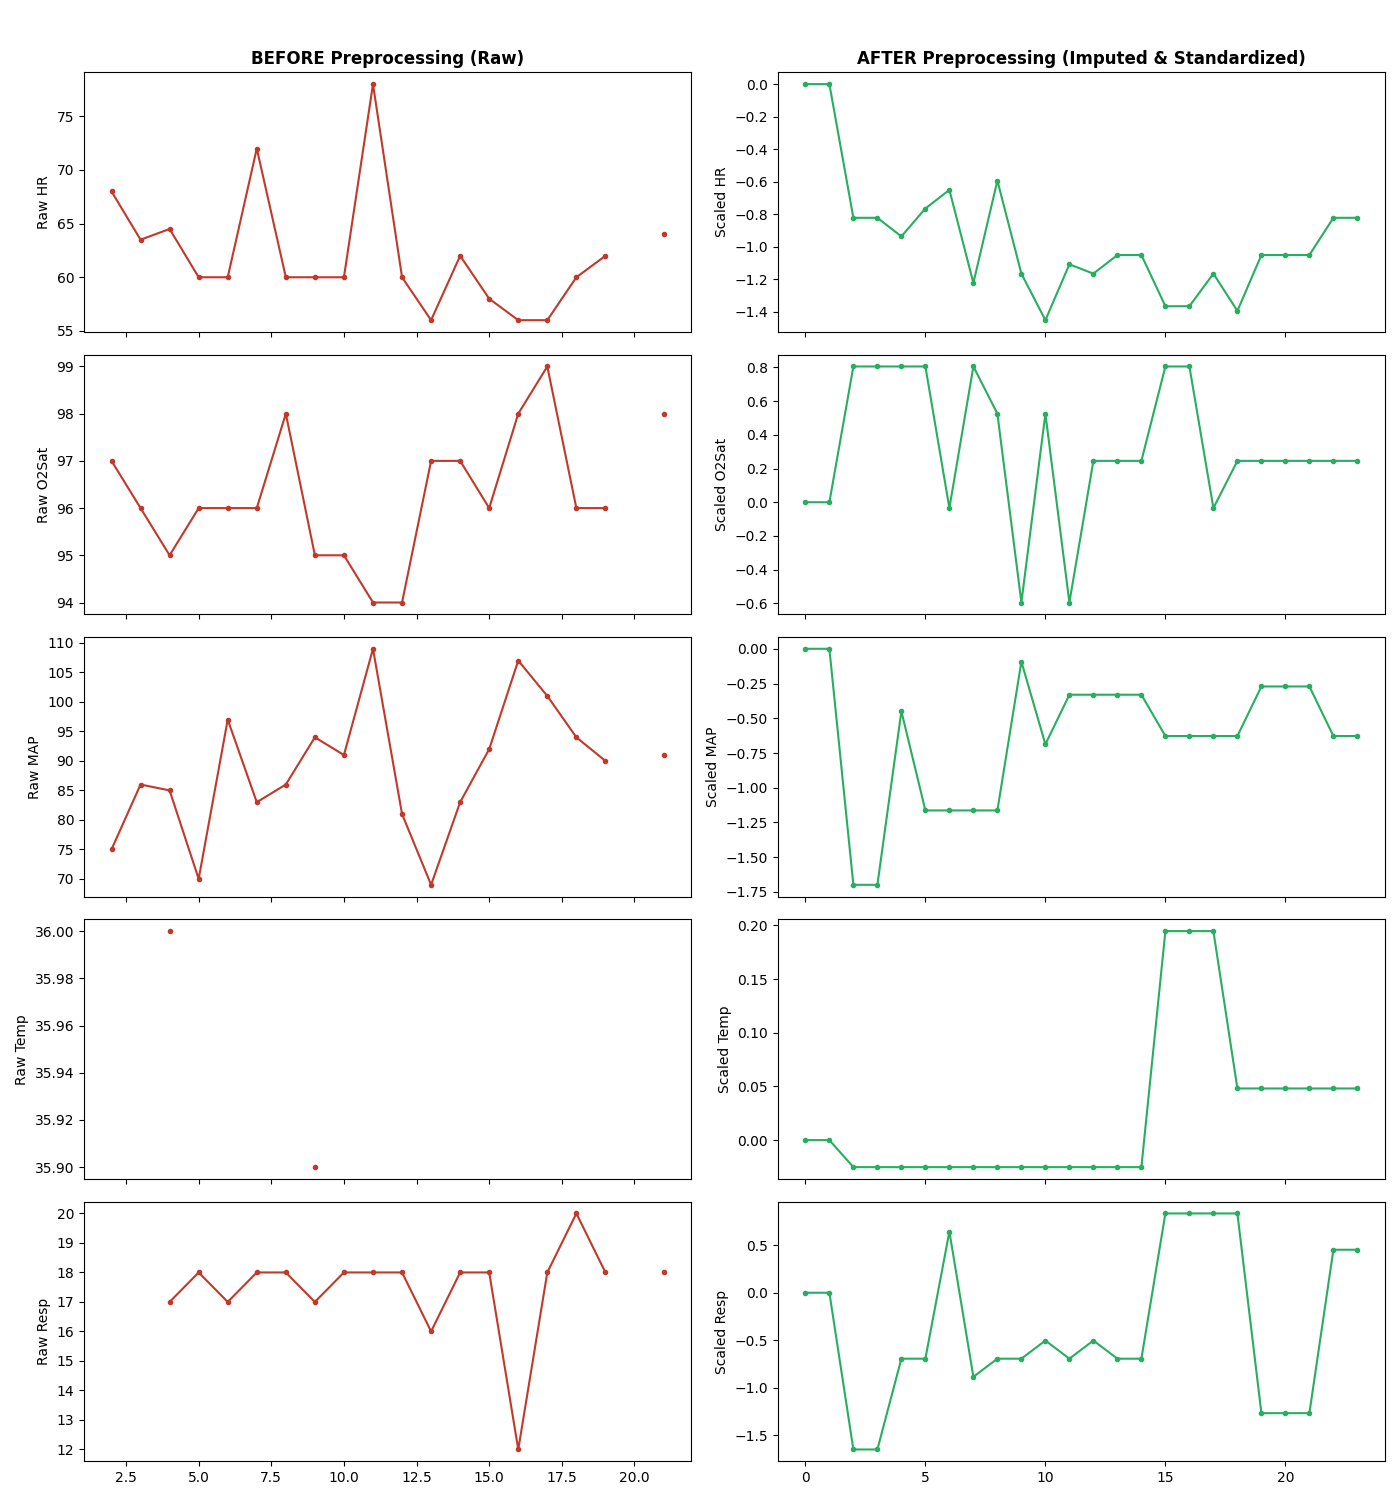
\includegraphics[width=\linewidth]{images/preprocessing_comparison.png}
\caption{Imputation \& Z-Score Normalization}
\end{subfigure}
\hfill
\begin{subfigure}[b]{0.48\textwidth}
\centering
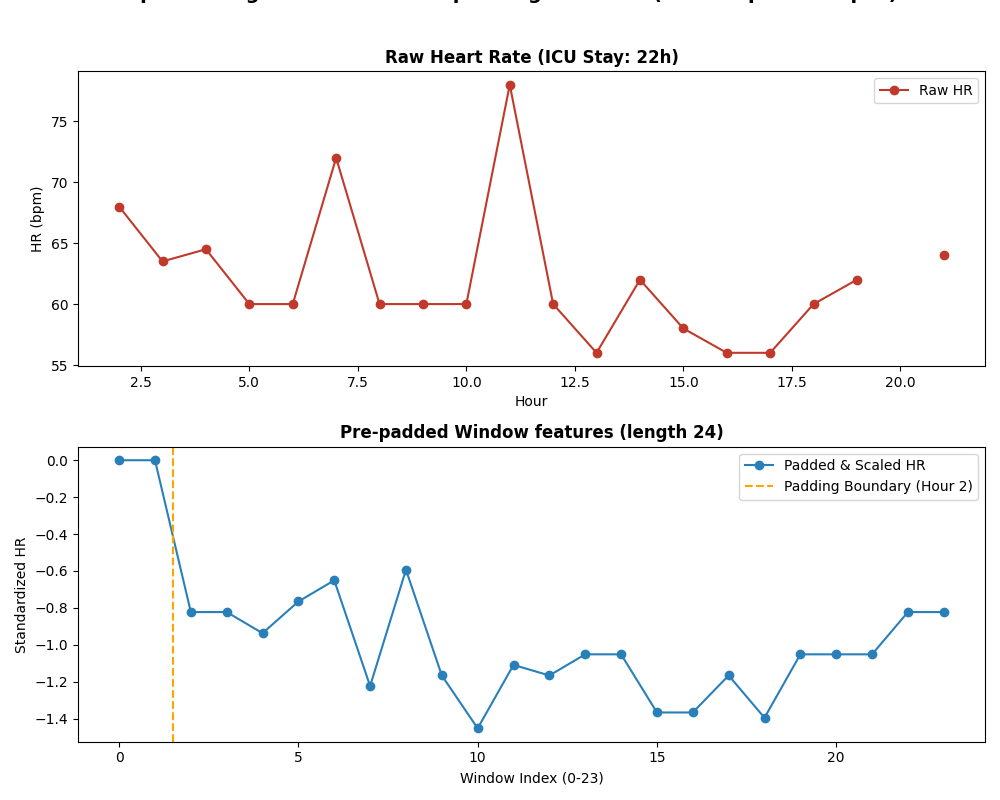
\includegraphics[width=\linewidth]{images/preprocessing_padding.png}
\caption{Zero Pre-Padding Validation ($T < 24$h)}
\end{subfigure}
\caption{Data preprocessing engineering pipeline validation.}
\label{fig:preprocessing_fig}
\end{figure*}

\section{Centralized Baseline BiLSTM Model}
We first train a Centralized Bidirectional LSTM model on the combined dataset as a reference benchmark. The network architecture consists of a 2-layer BiLSTM backbone (hidden dimension = 64, dropout = 0.3) followed by a dense classification layer.

\subsection{Weighted Loss Formulation}
Given the severe class imbalance in ICU sepsis occurrence ($\sim 2.5\%$ positive window ratio), standard Binary Cross-Entropy (BCE) loss biases models toward false negative predictions. We implement a dynamic positive class weight:
$$\mathcal{L}_{\text{BCE}} = -\left[ w_{\text{pos}} \cdot y \log \sigma(\hat{y}) + (1 - y) \log (1 - \sigma(\hat{y})) \right]$$
where $w_{\text{pos}} = \frac{N_{\text{neg}}}{N_{\text{pos}}} \approx 37.17$.

\subsection{Baseline Inference Performance}
The centralized model early-stopped at Epoch 9 as validation AUROC peaked at 0.8232. Final test set metrics are detailed in Table~\ref{tab:metrics}. Figure~\ref{fig:baseline_fig} presents the test ROC curve (AUROC = 0.8058) and confusion matrix heatmap.

\begin{table}[htbp]
\caption{Centralized Baseline Test Evaluation}
\label{tab:metrics}
\centering
\begin{tabular}{lc}
\toprule
\textbf{Metric} & \textbf{Centralized Baseline} \\
\midrule
Accuracy & 75.09\% \\
Precision & 7.14\% \\
Recall (Sensitivity) & 72.17\% \\
F1 Score & 0.1300 \\
\textbf{AUROC} & \textbf{0.8058} \\
\bottomrule
\end{tabular}
\end{table}

\begin{figure*}[t]
\centering
\begin{subfigure}[b]{0.48\textwidth}
\centering
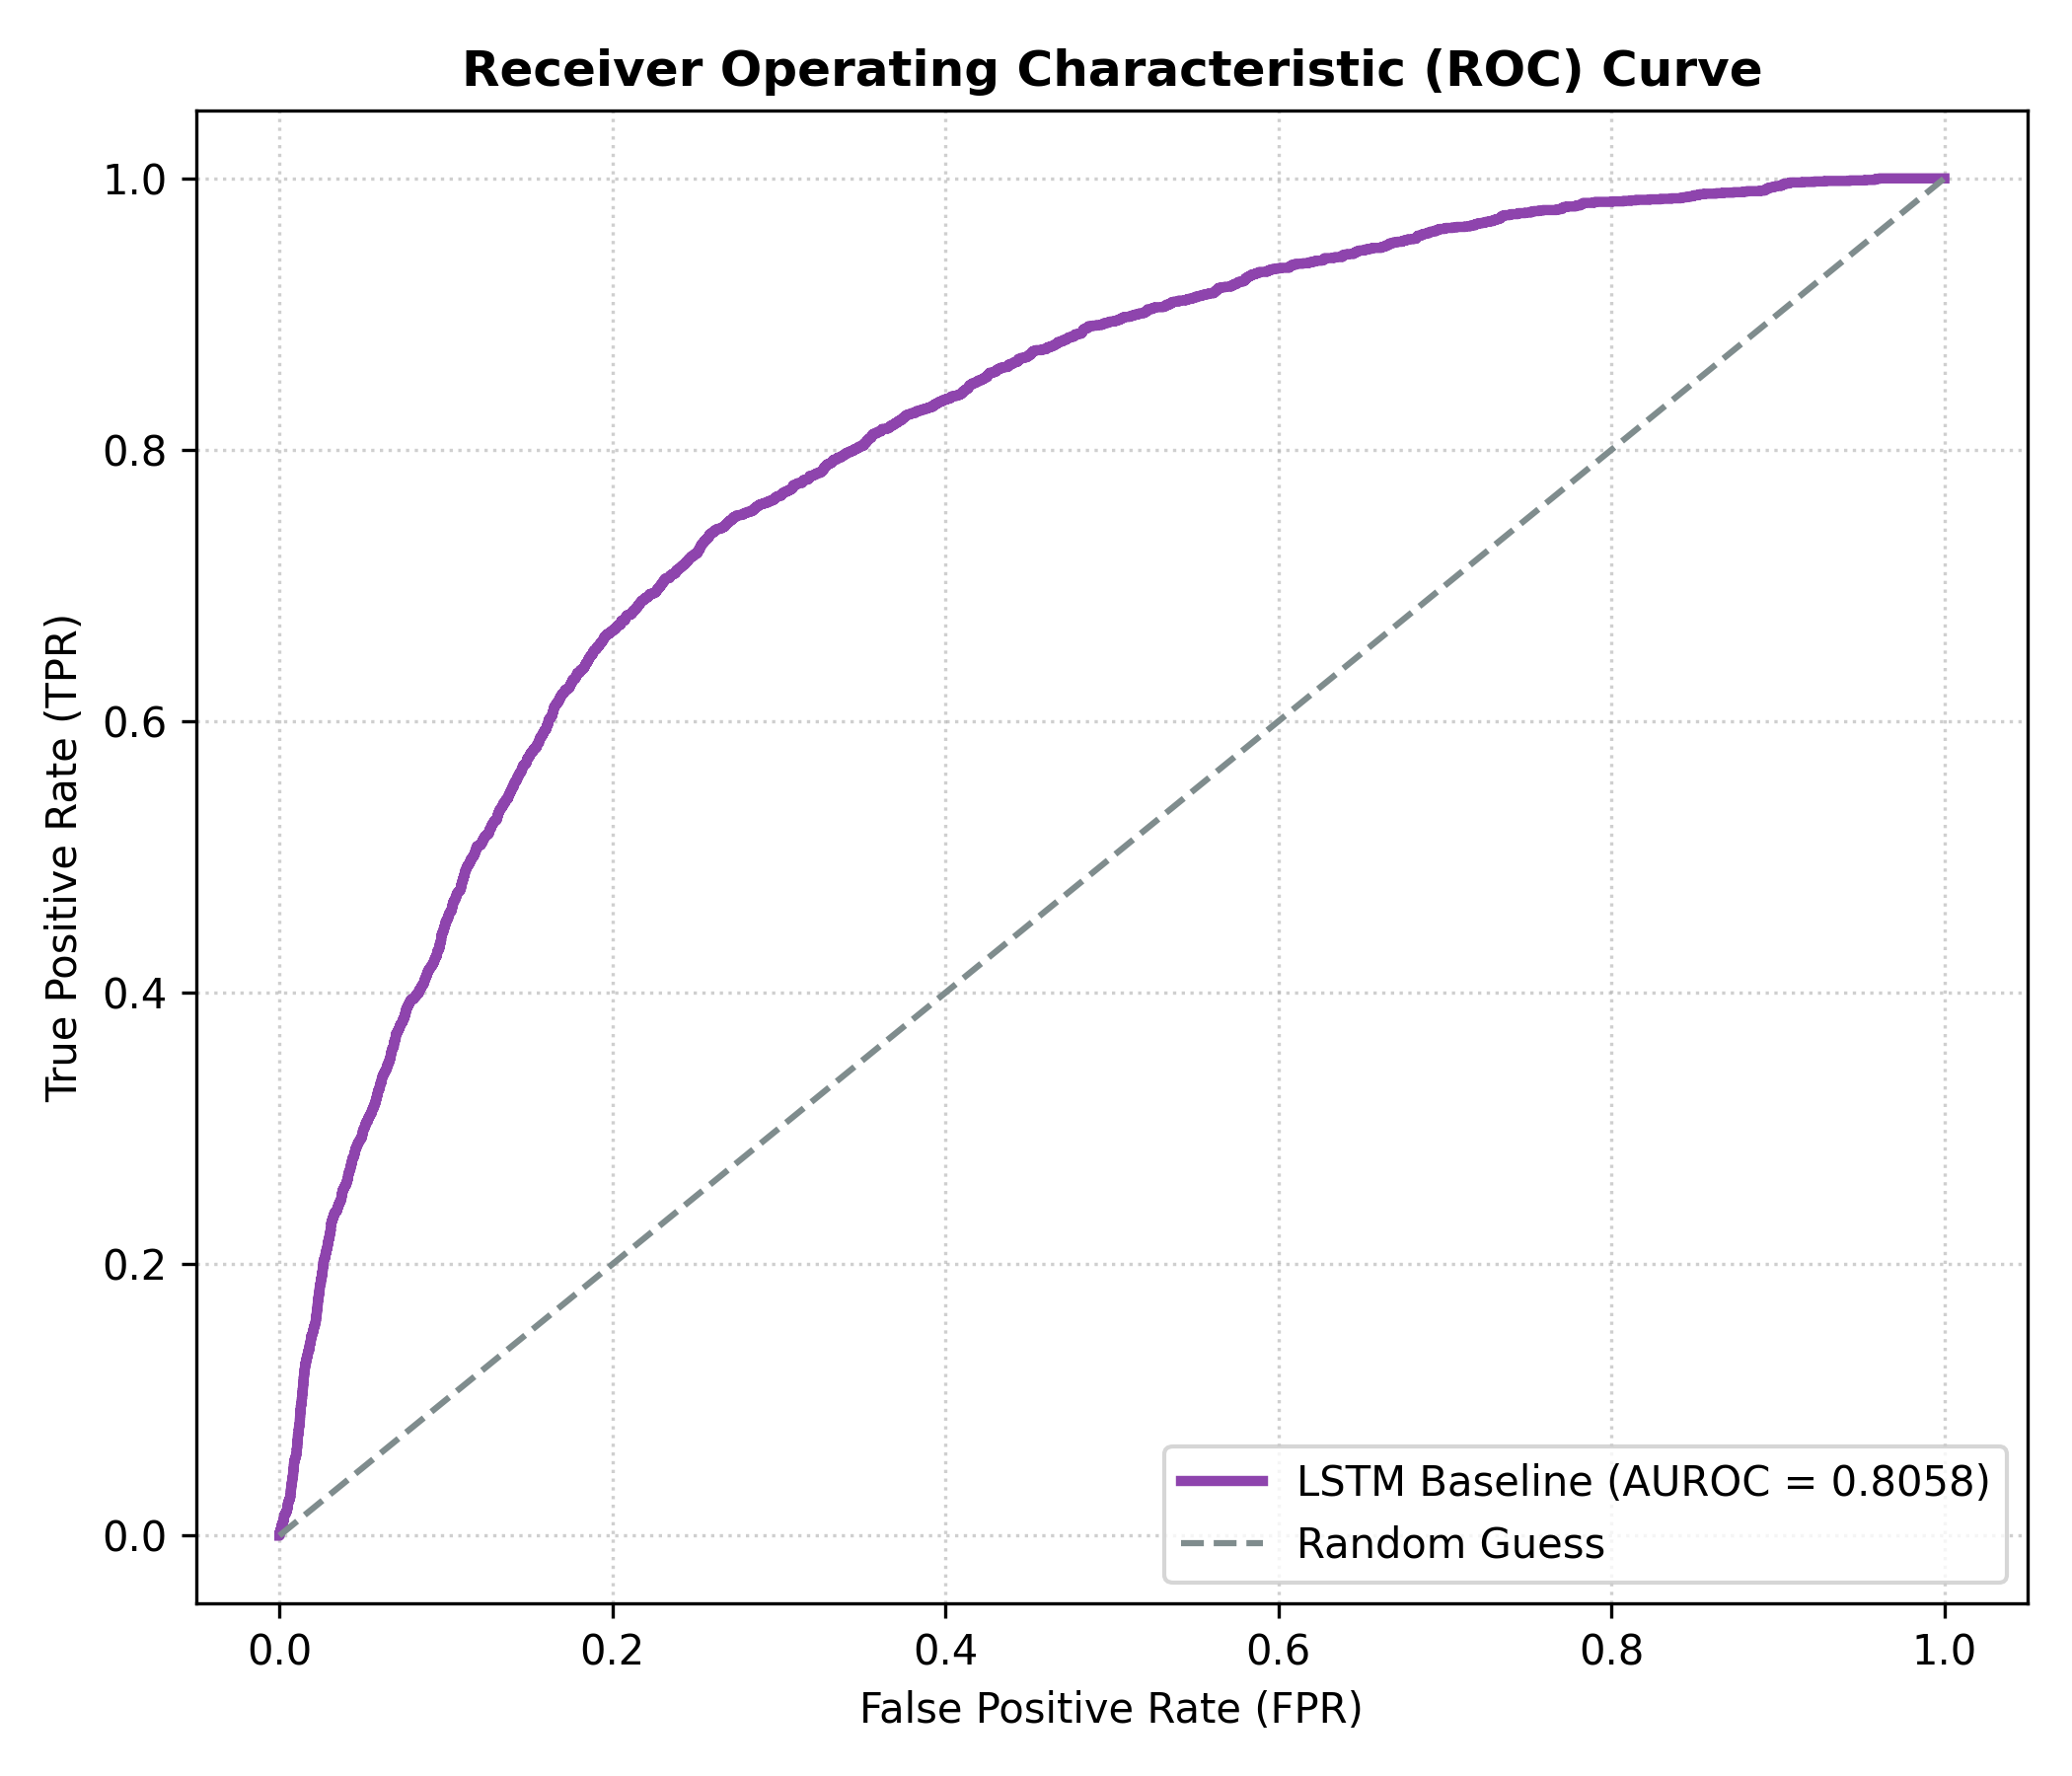
\includegraphics[width=\linewidth]{images/baseline_roc.png}
\caption{Centralized Test ROC Curve}
\end{subfigure}
\hfill
\begin{subfigure}[b]{0.48\textwidth}
\centering
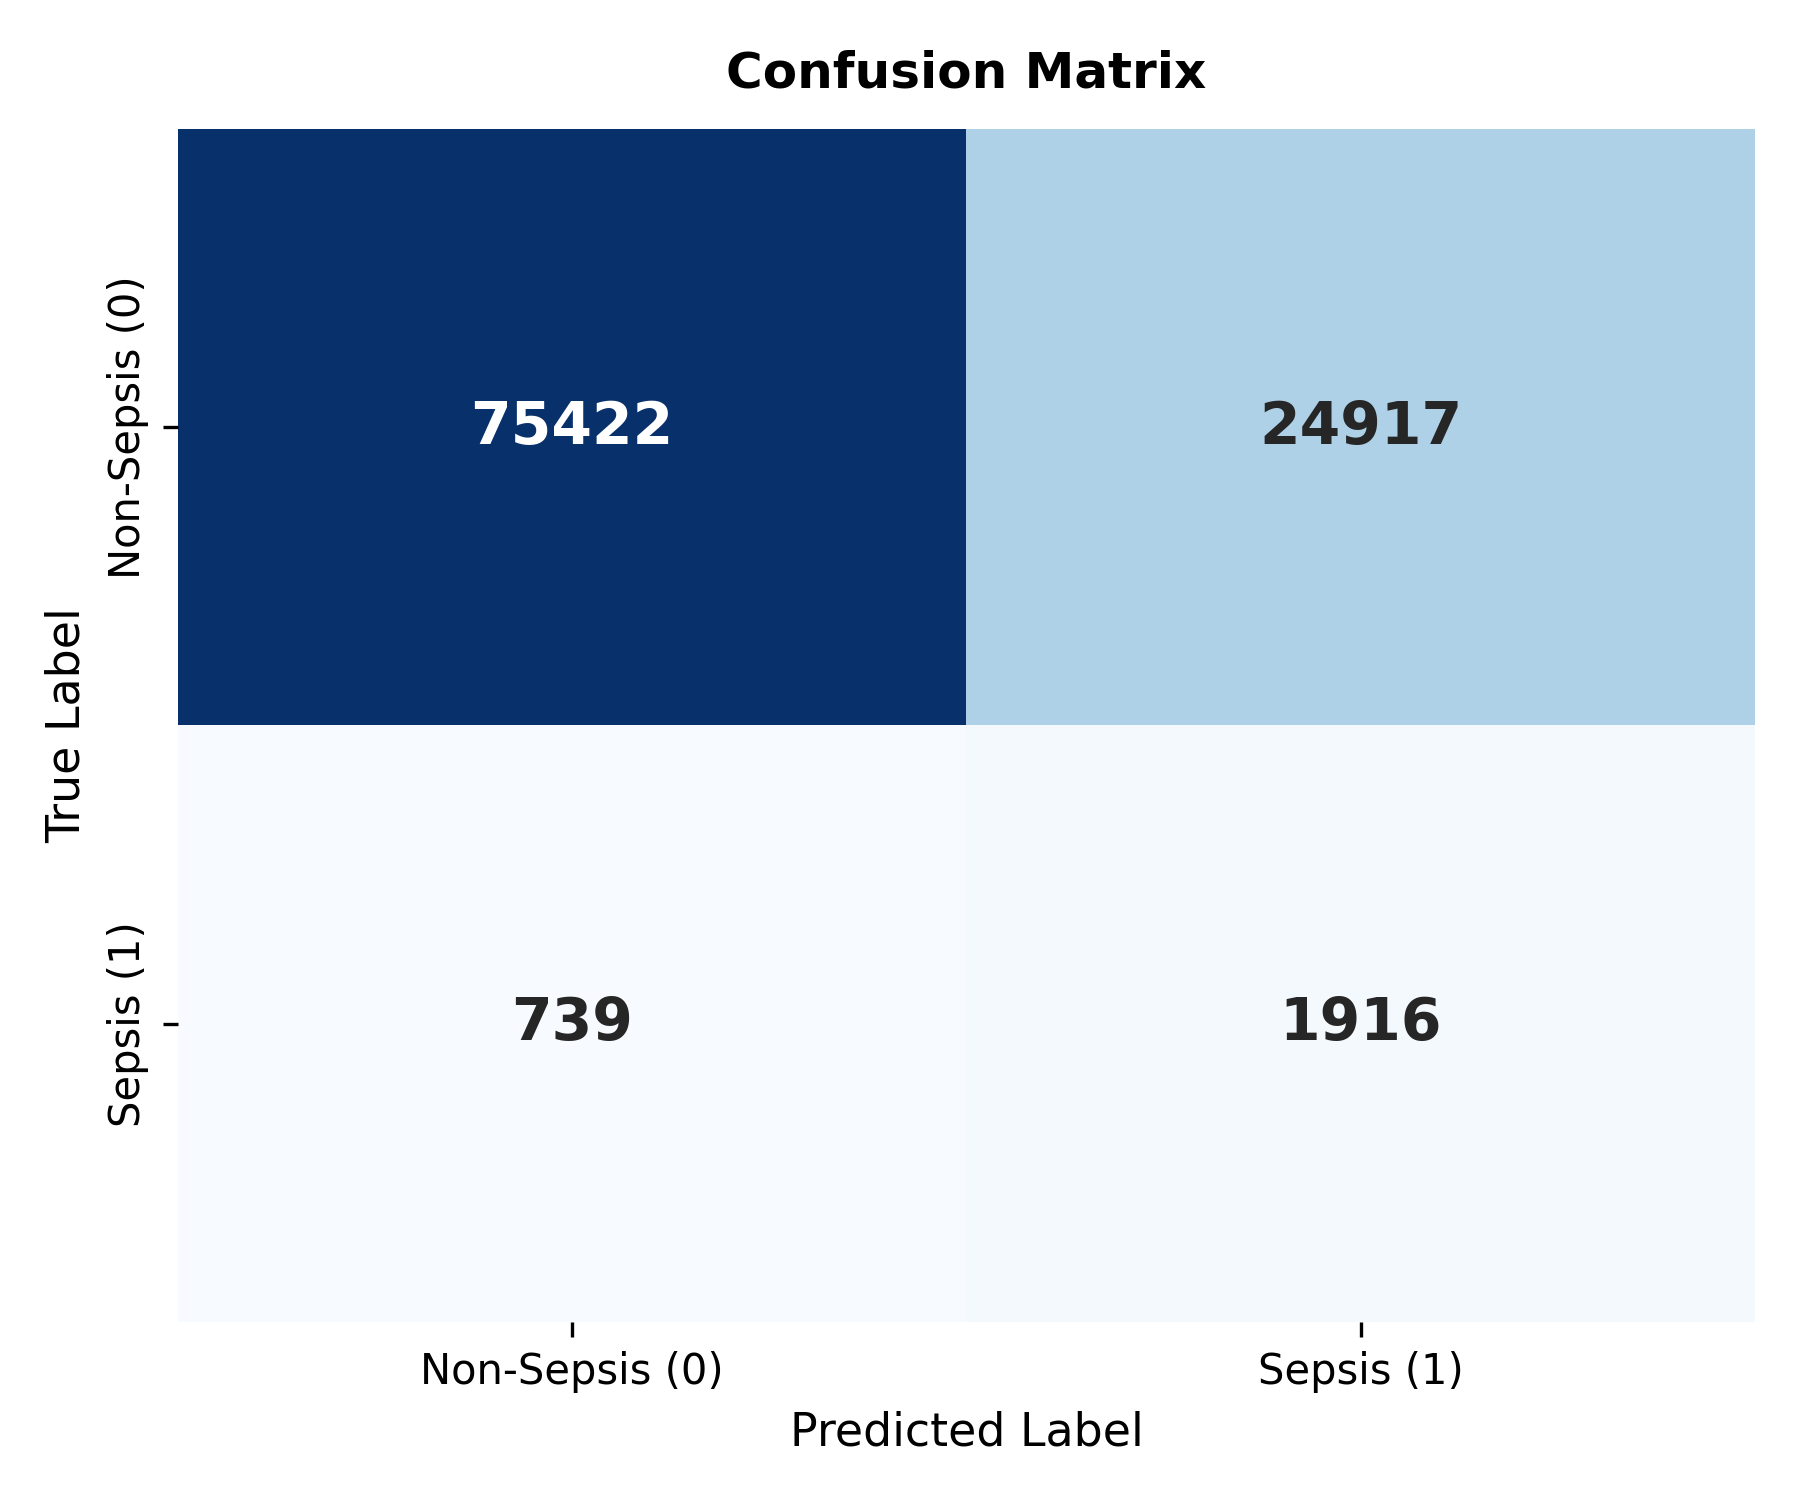
\includegraphics[width=\linewidth]{images/baseline_confusion_matrix.png}
\caption{Test Confusion Matrix Heatmap}
\end{subfigure}
\caption{Centralized Baseline BiLSTM test evaluation.}
\label{fig:baseline_fig}
\end{figure*}

\section{Federated Learning via FedAvg}
To enforce data privacy across healthcare institutions, we convert the model into a decentralized federated system using Federated Averaging (FedAvg) \cite{mcmahan2017}.

\subsection{Non-IID Clinical Node Simulation}
We partition the PhysioNet dataset across three decentralized hospital client nodes simulating real-world patient demographic and institutional heterogeneity:
\begin{itemize}
\item \textbf{Hospital 1 (Client Node 0, Age $<$ 60)}: 92,613 training sequence samples, 3.24\% positive rate.
\item \textbf{Hospital 2 (Client Node 1, Age $\ge$ 60)}: 151,916 training sequence samples, 3.09\% positive rate.
\item \textbf{Hospital 3 (Client Node 2, Regional Node)}: 233,140 training sequence samples, 2.07\% positive rate.
\end{itemize}

\subsection{Federated Optimization Loop}
In each communication round $t$, the central server broadcasts global model weights $W_{\text{global}}^t$. Clients perform $E=2$ local SGD epochs, and the server aggregates updates:
$$W_{\text{global}}^{t+1} = \sum_{k=1}^K \frac{n_k}{N} W_k^{t+1}$$
where $n_k$ is the local sample size of client node $k$ and $N = \sum n_k$.

\subsection{Results and Baseline Degradation Analysis}
FedAvg training early-stopped at round 7. Figure~\ref{fig:fed_curves} shows global validation loss and AUROC curves across rounds. Table~\ref{tab:comparison} compares FedAvg against the Centralized Baseline.

\begin{figure*}[t]
\centering
\begin{subfigure}[b]{0.48\textwidth}
\centering
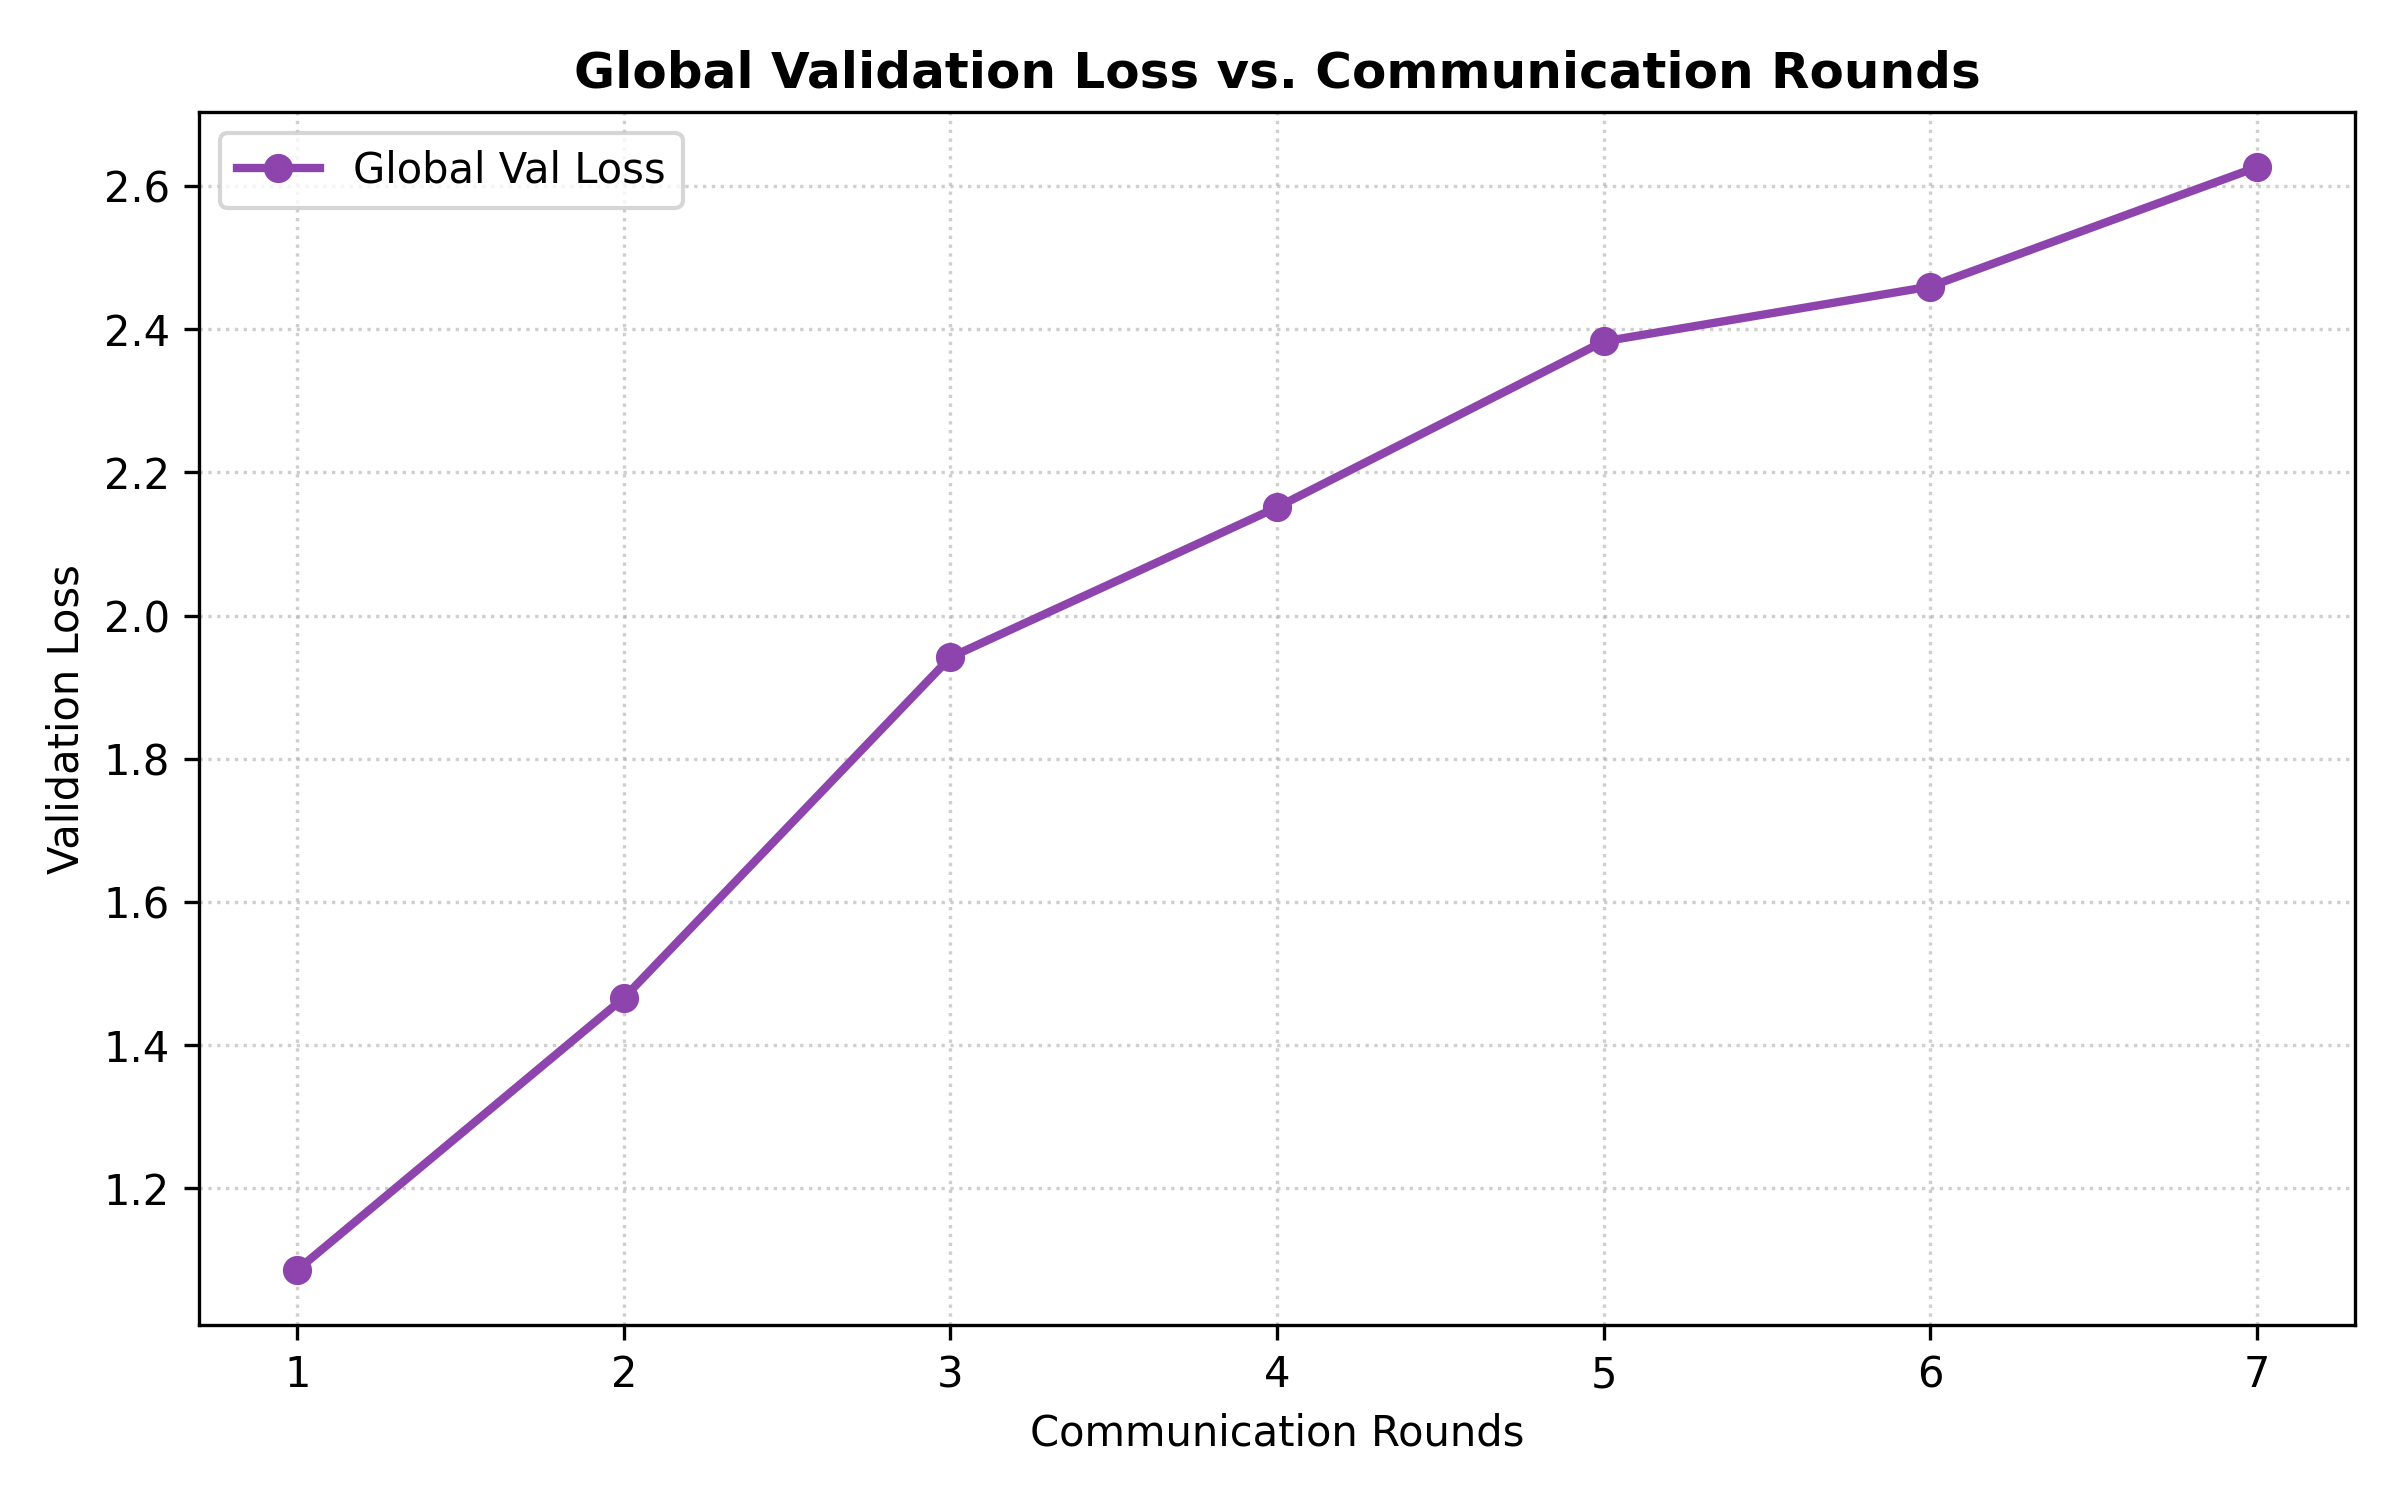
\includegraphics[width=\linewidth]{images/federated_rounds_loss.png}
\caption{Validation Loss Across Rounds}
\end{subfigure}
\hfill
\begin{subfigure}[b]{0.48\textwidth}
\centering
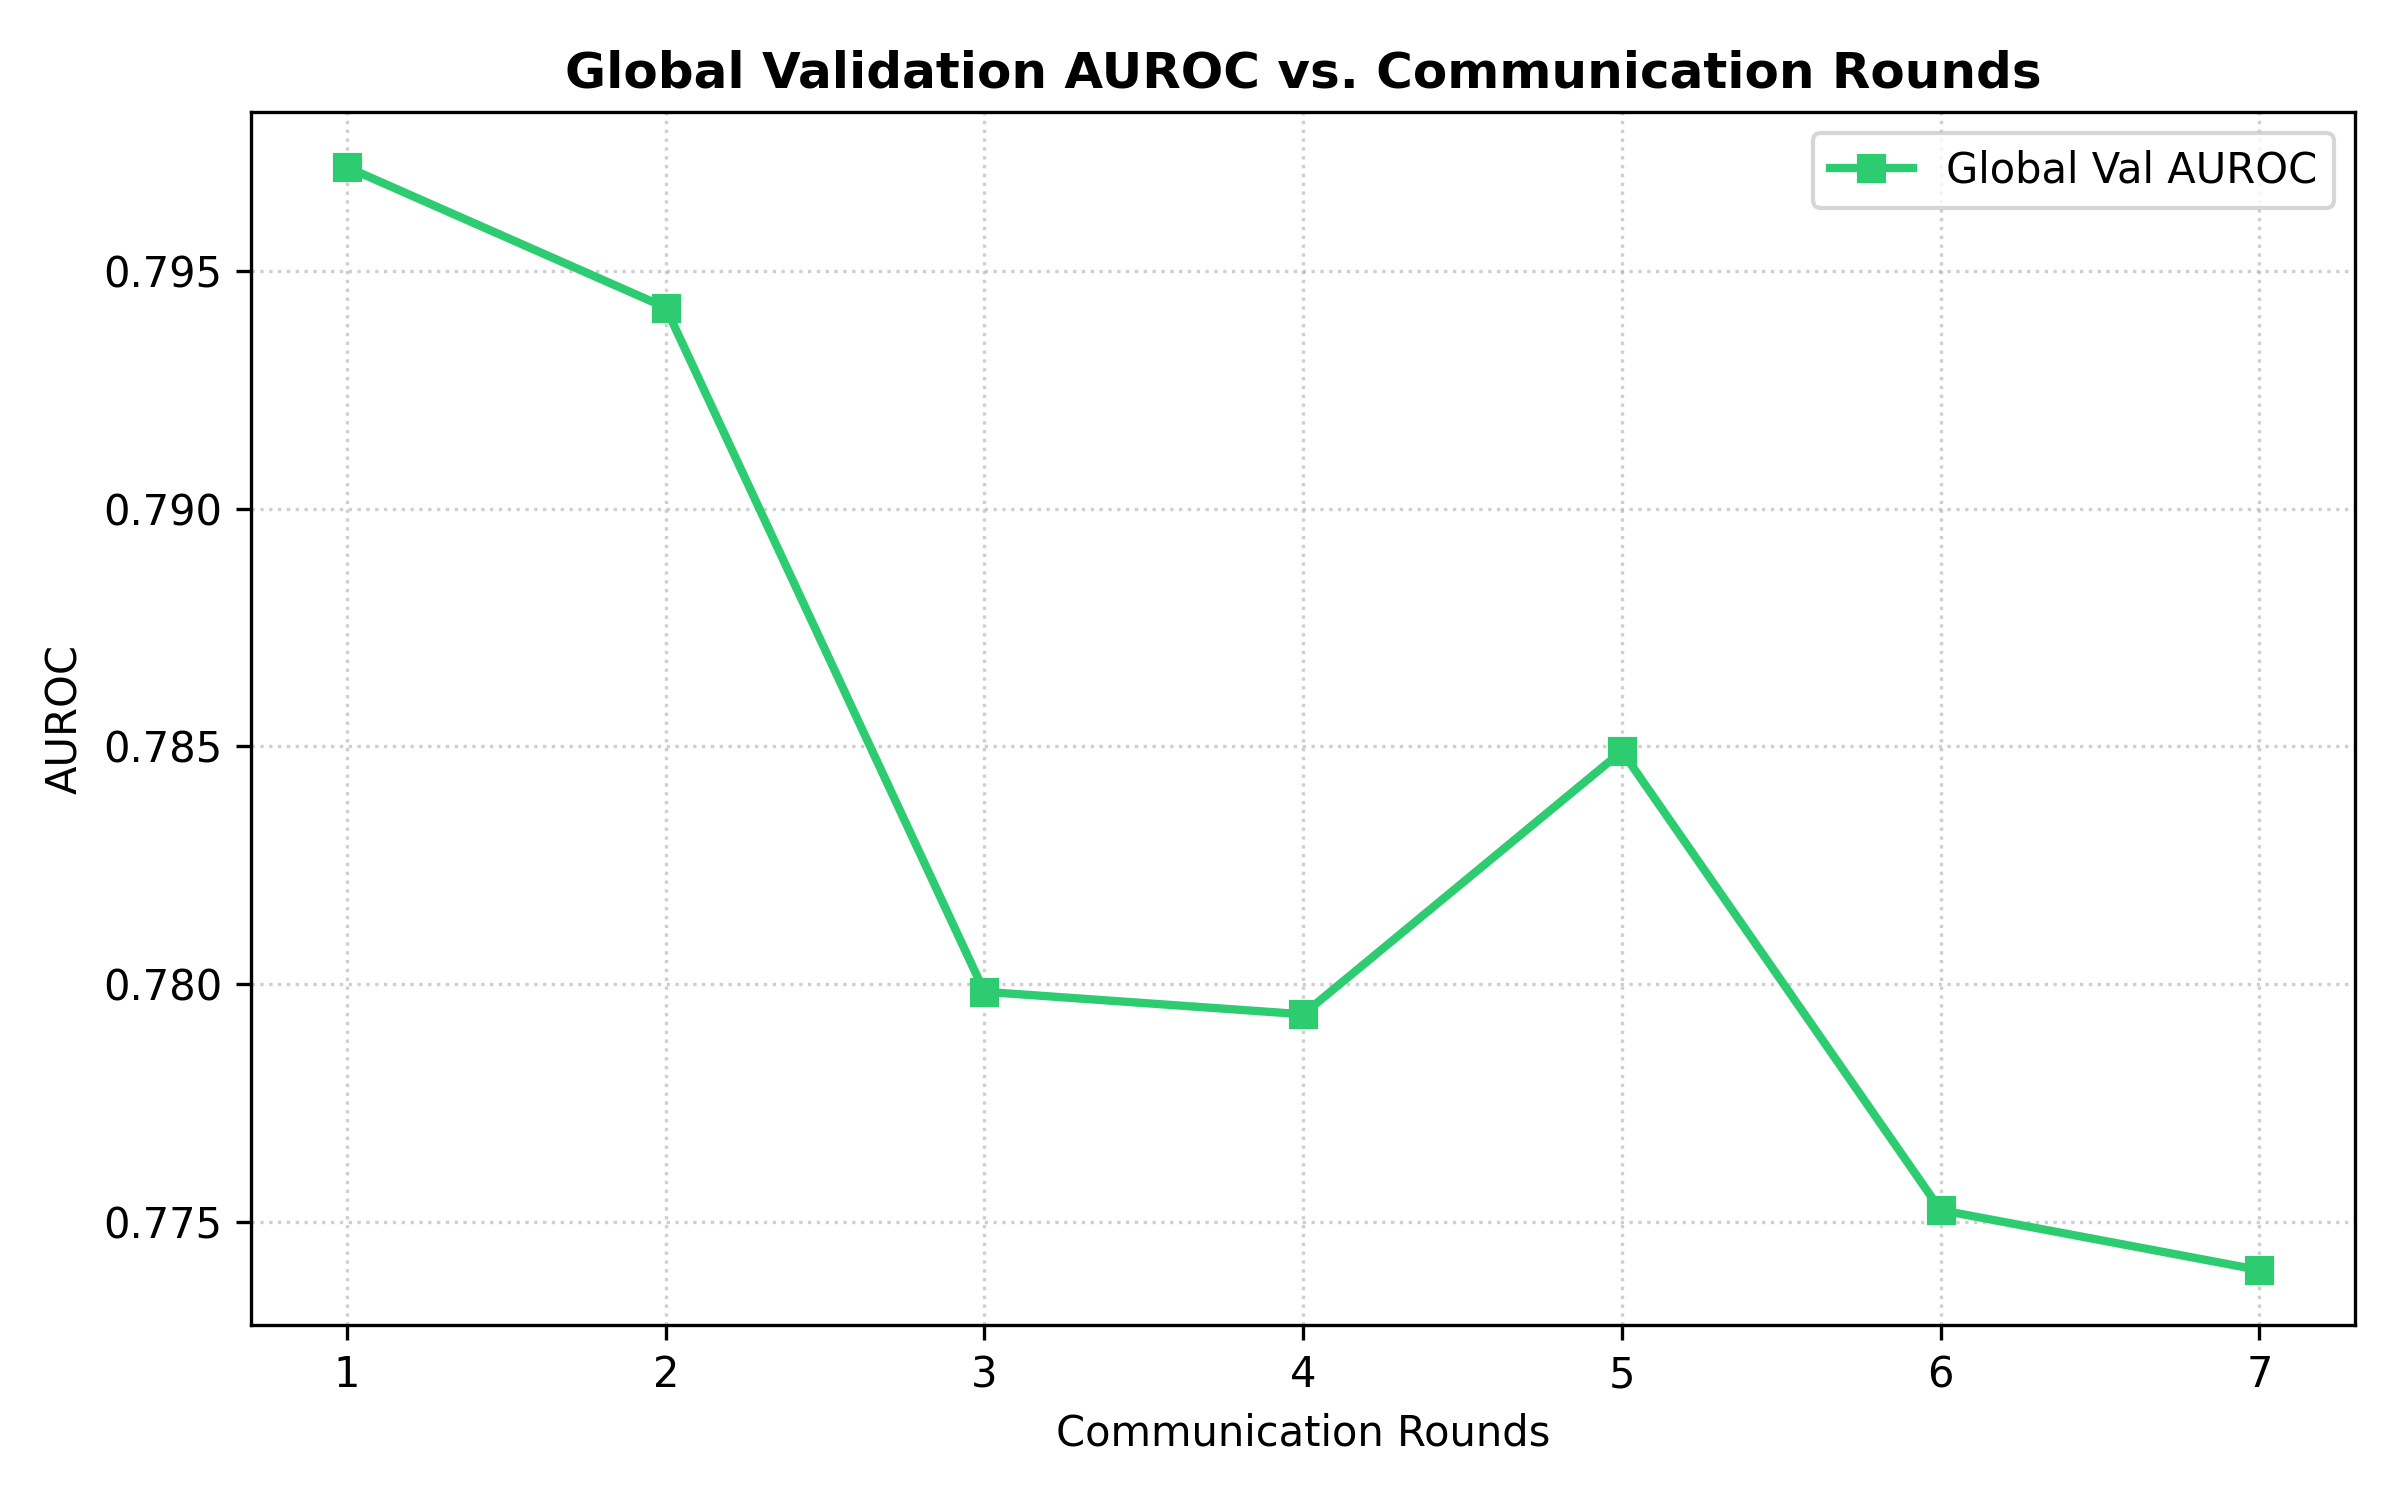
\includegraphics[width=\linewidth]{images/federated_rounds_auroc.png}
\caption{Validation AUROC Across Rounds}
\end{subfigure}
\caption{FedAvg global model performance across 10 communication rounds.}
\label{fig:fed_curves}
\end{figure*}

\begin{table}[htbp]
\caption{Comparative Test Results: Centralized vs. FedAvg}
\label{tab:comparison}
\centering
\begin{tabular}{lccc}
\toprule
\textbf{Metric} & \textbf{Centralized} & \textbf{FedAvg} & \textbf{Difference} \\
\midrule
Accuracy & 75.09\% & 75.94\% & +0.85\% \\
Precision & 7.14\% & 6.94\% & -0.20\% \\
Recall & 72.17\% & 67.19\% & -4.97\% \\
F1 Score & 0.1300 & 0.1259 & -0.0041 \\
\textbf{AUROC} & \textbf{0.8058} & \textbf{0.7844} & \textbf{-0.0214} \\
\bottomrule
\end{tabular}
\end{table}

Due to client Non-IID heterogeneity, FedAvg exhibits a **2.14\% drop in test AUROC** (0.7844 vs 0.8058) and a **4.97\% drop in Recall**, confirming that a single static global consensus model struggles under institutional demographic shifts. Figure~\ref{fig:fed_roc_cm} plots the FedAvg ROC curve and confusion matrix.

\begin{figure*}[t]
\centering
\begin{subfigure}[b]{0.48\textwidth}
\centering
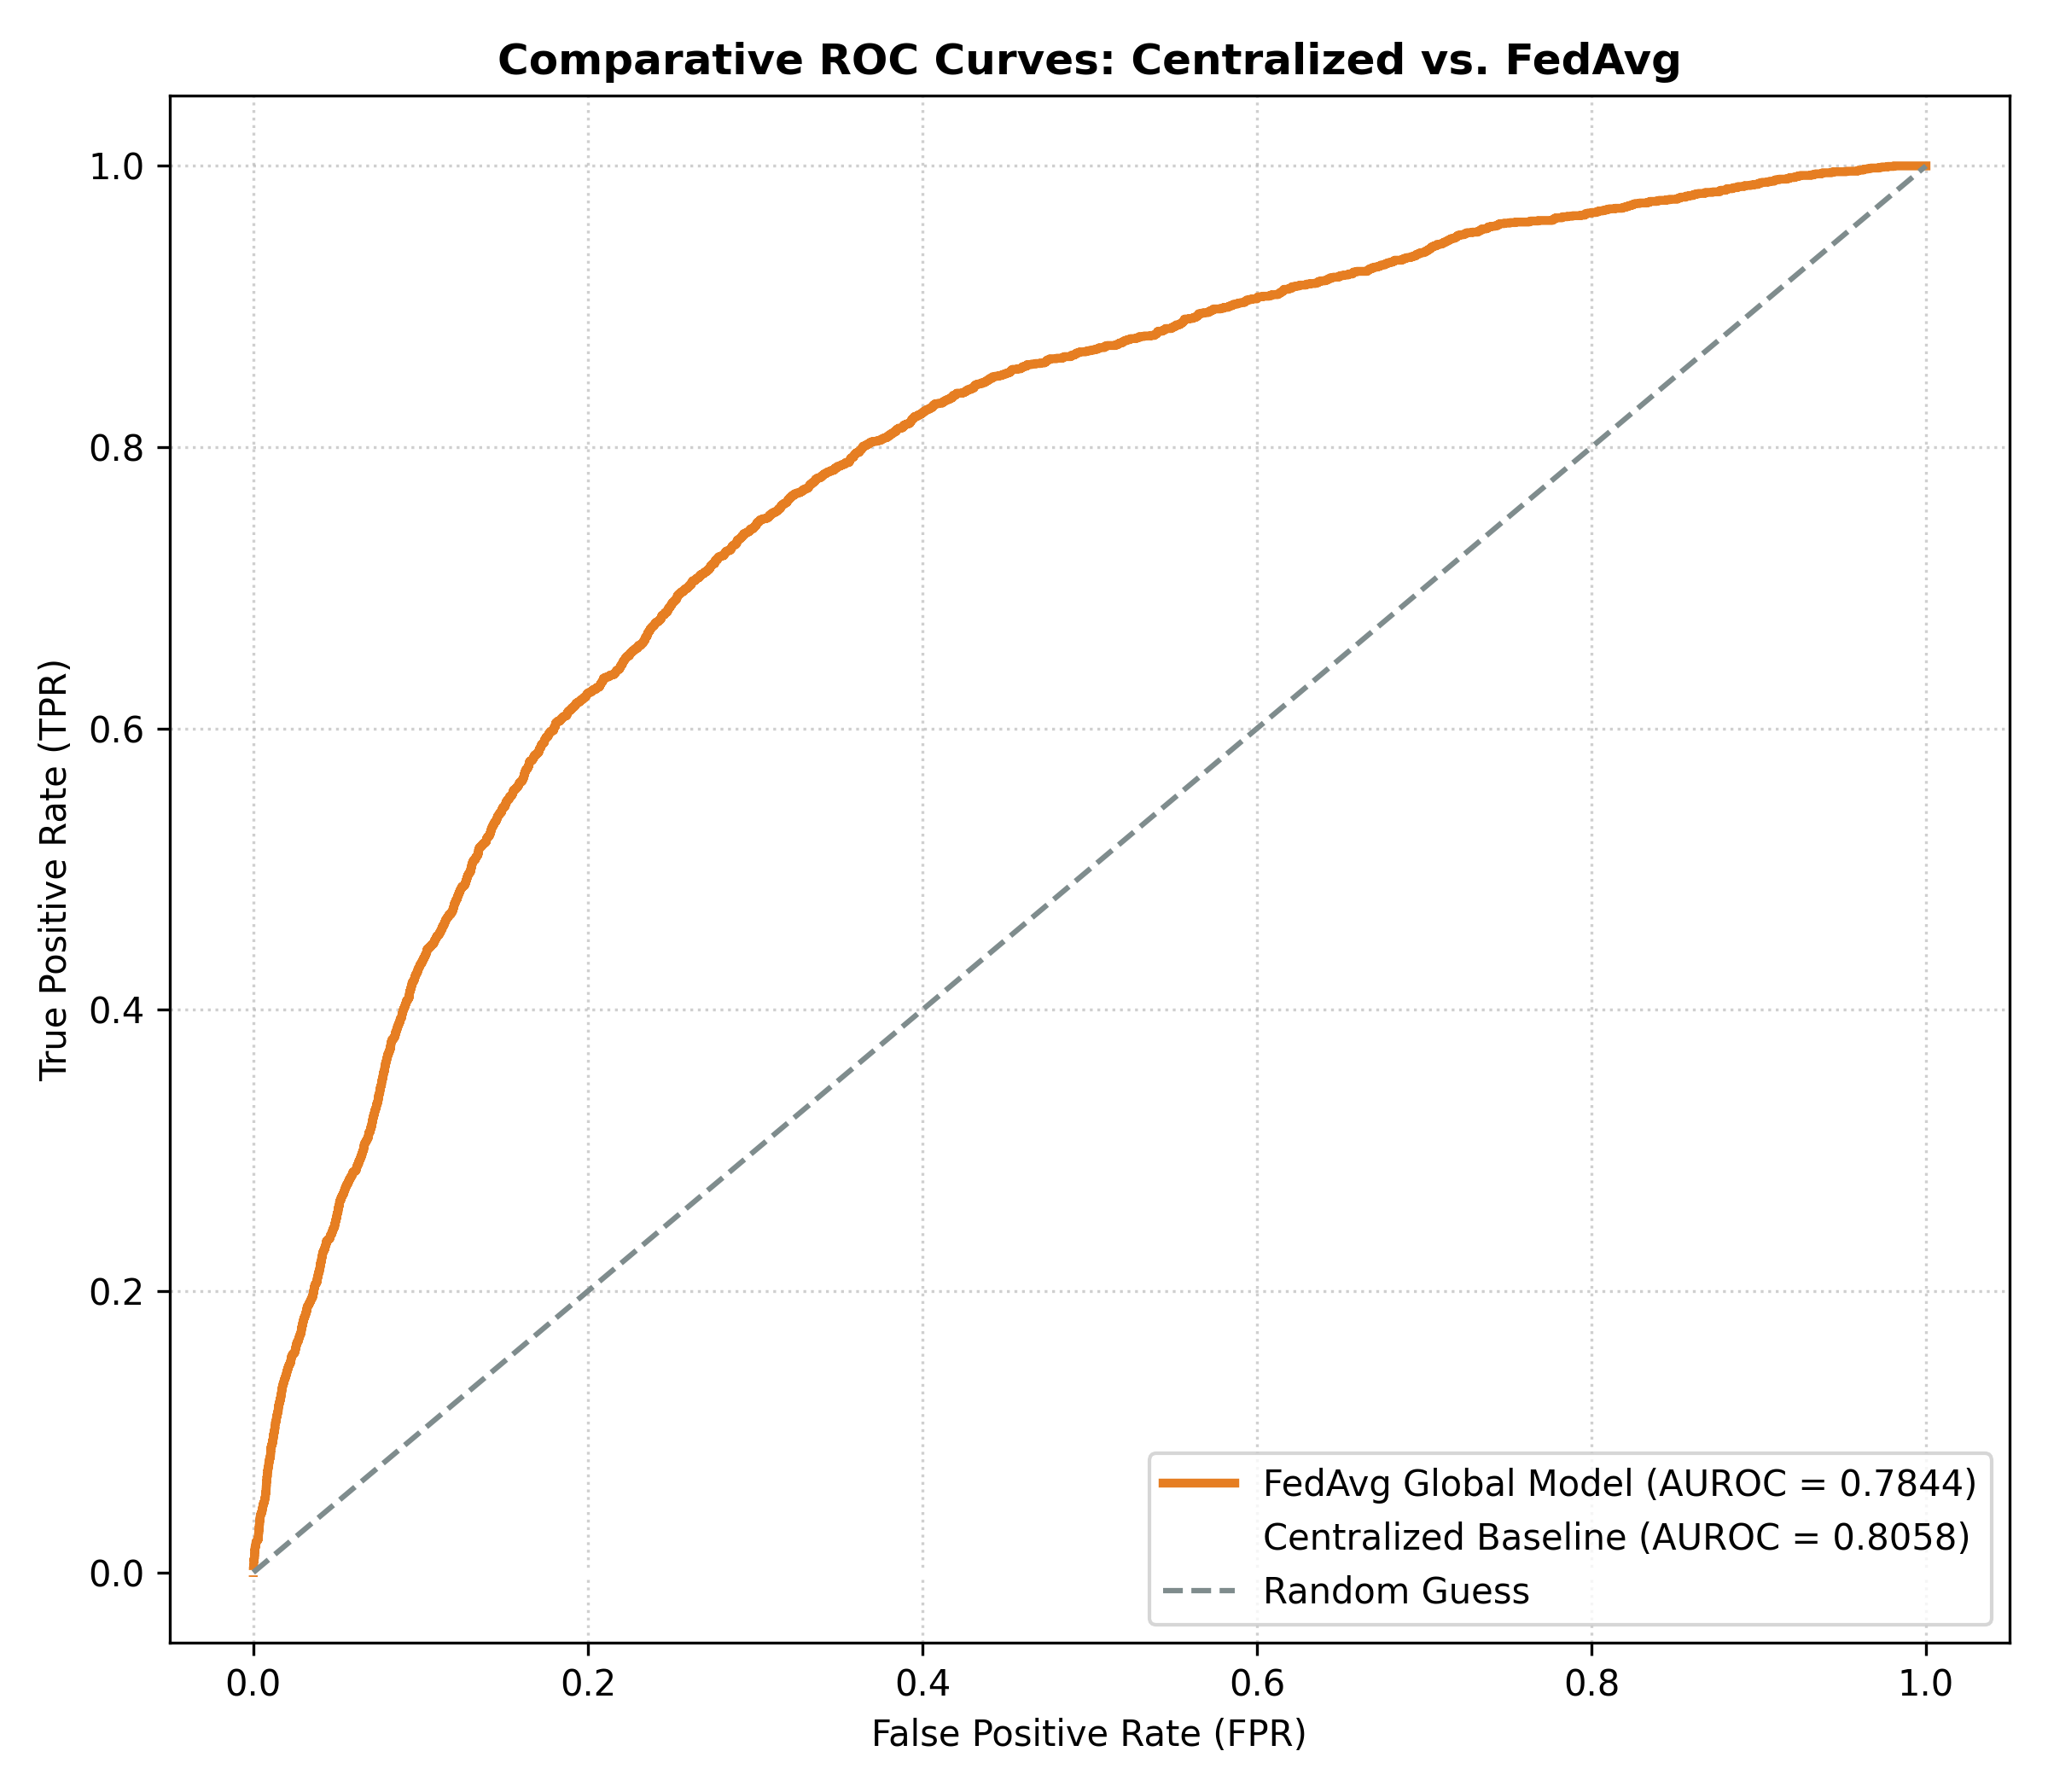
\includegraphics[width=\linewidth]{images/federated_comparative_roc.png}
\caption{FedAvg Test ROC Overlay}
\end{subfigure}
\hfill
\begin{subfigure}[b]{0.48\textwidth}
\centering
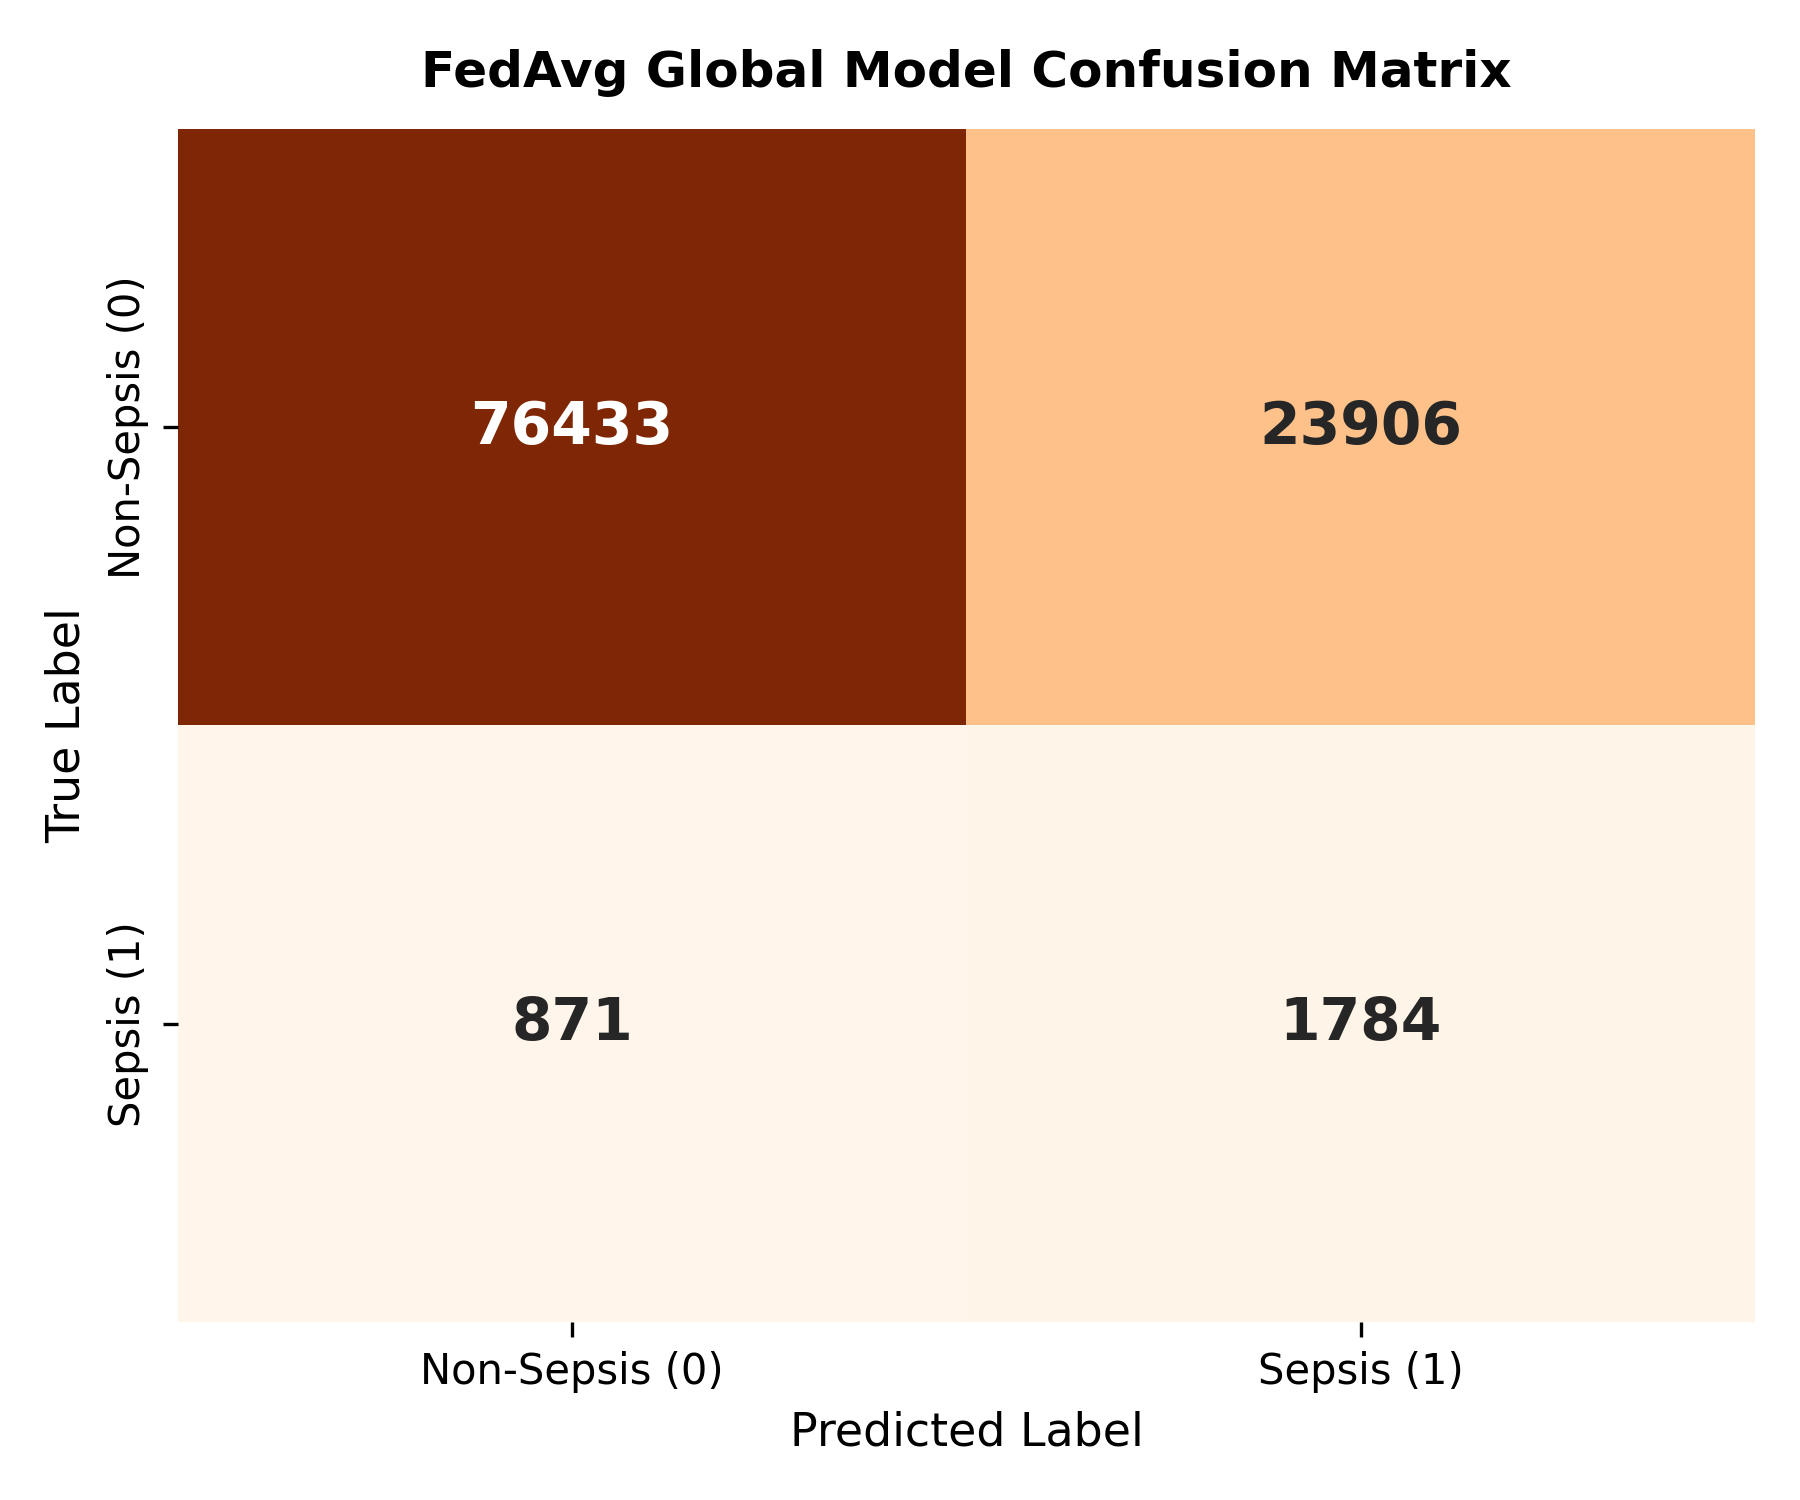
\includegraphics[width=\linewidth]{images/federated_confusion_matrix.png}
\caption{FedAvg Confusion Matrix}
\end{subfigure}
\caption{FedAvg global model test evaluation.}
\label{fig:fed_roc_cm}
\end{figure*}

\section{Federated Learning via FedProx}
To counteract weight divergence caused by Non-IID data distributions, we deploy FedProx \cite{li2020fedprox}.

\subsection{Proximal Regularization Formulation}
FedProx modifies local client loss functions by adding a proximal penalty:
$$\mathcal{L}_{\text{local}}(w; w_{\text{global}}^t) = \mathcal{L}_{\text{BCE}}(w) + \frac{\mu}{2} \sum_{p} \| w_p - (w_{\text{global}}^t)_p \|_2^2$$
We configure $\mu = 0.01$, constraining client weights from drifting too far from central consensus.

\subsection{Results and Three-Way Benchmarking}
FedProx early-stopped at round 8, with validation AUROC peaking at 0.8062 in Round 2. Figure~\ref{fig:fedprox_curves} presents validation metrics across rounds, and Table~\ref{tab:threeway} details three-way comparative performance.

\begin{figure*}[t]
\centering
\begin{subfigure}[b]{0.48\textwidth}
\centering
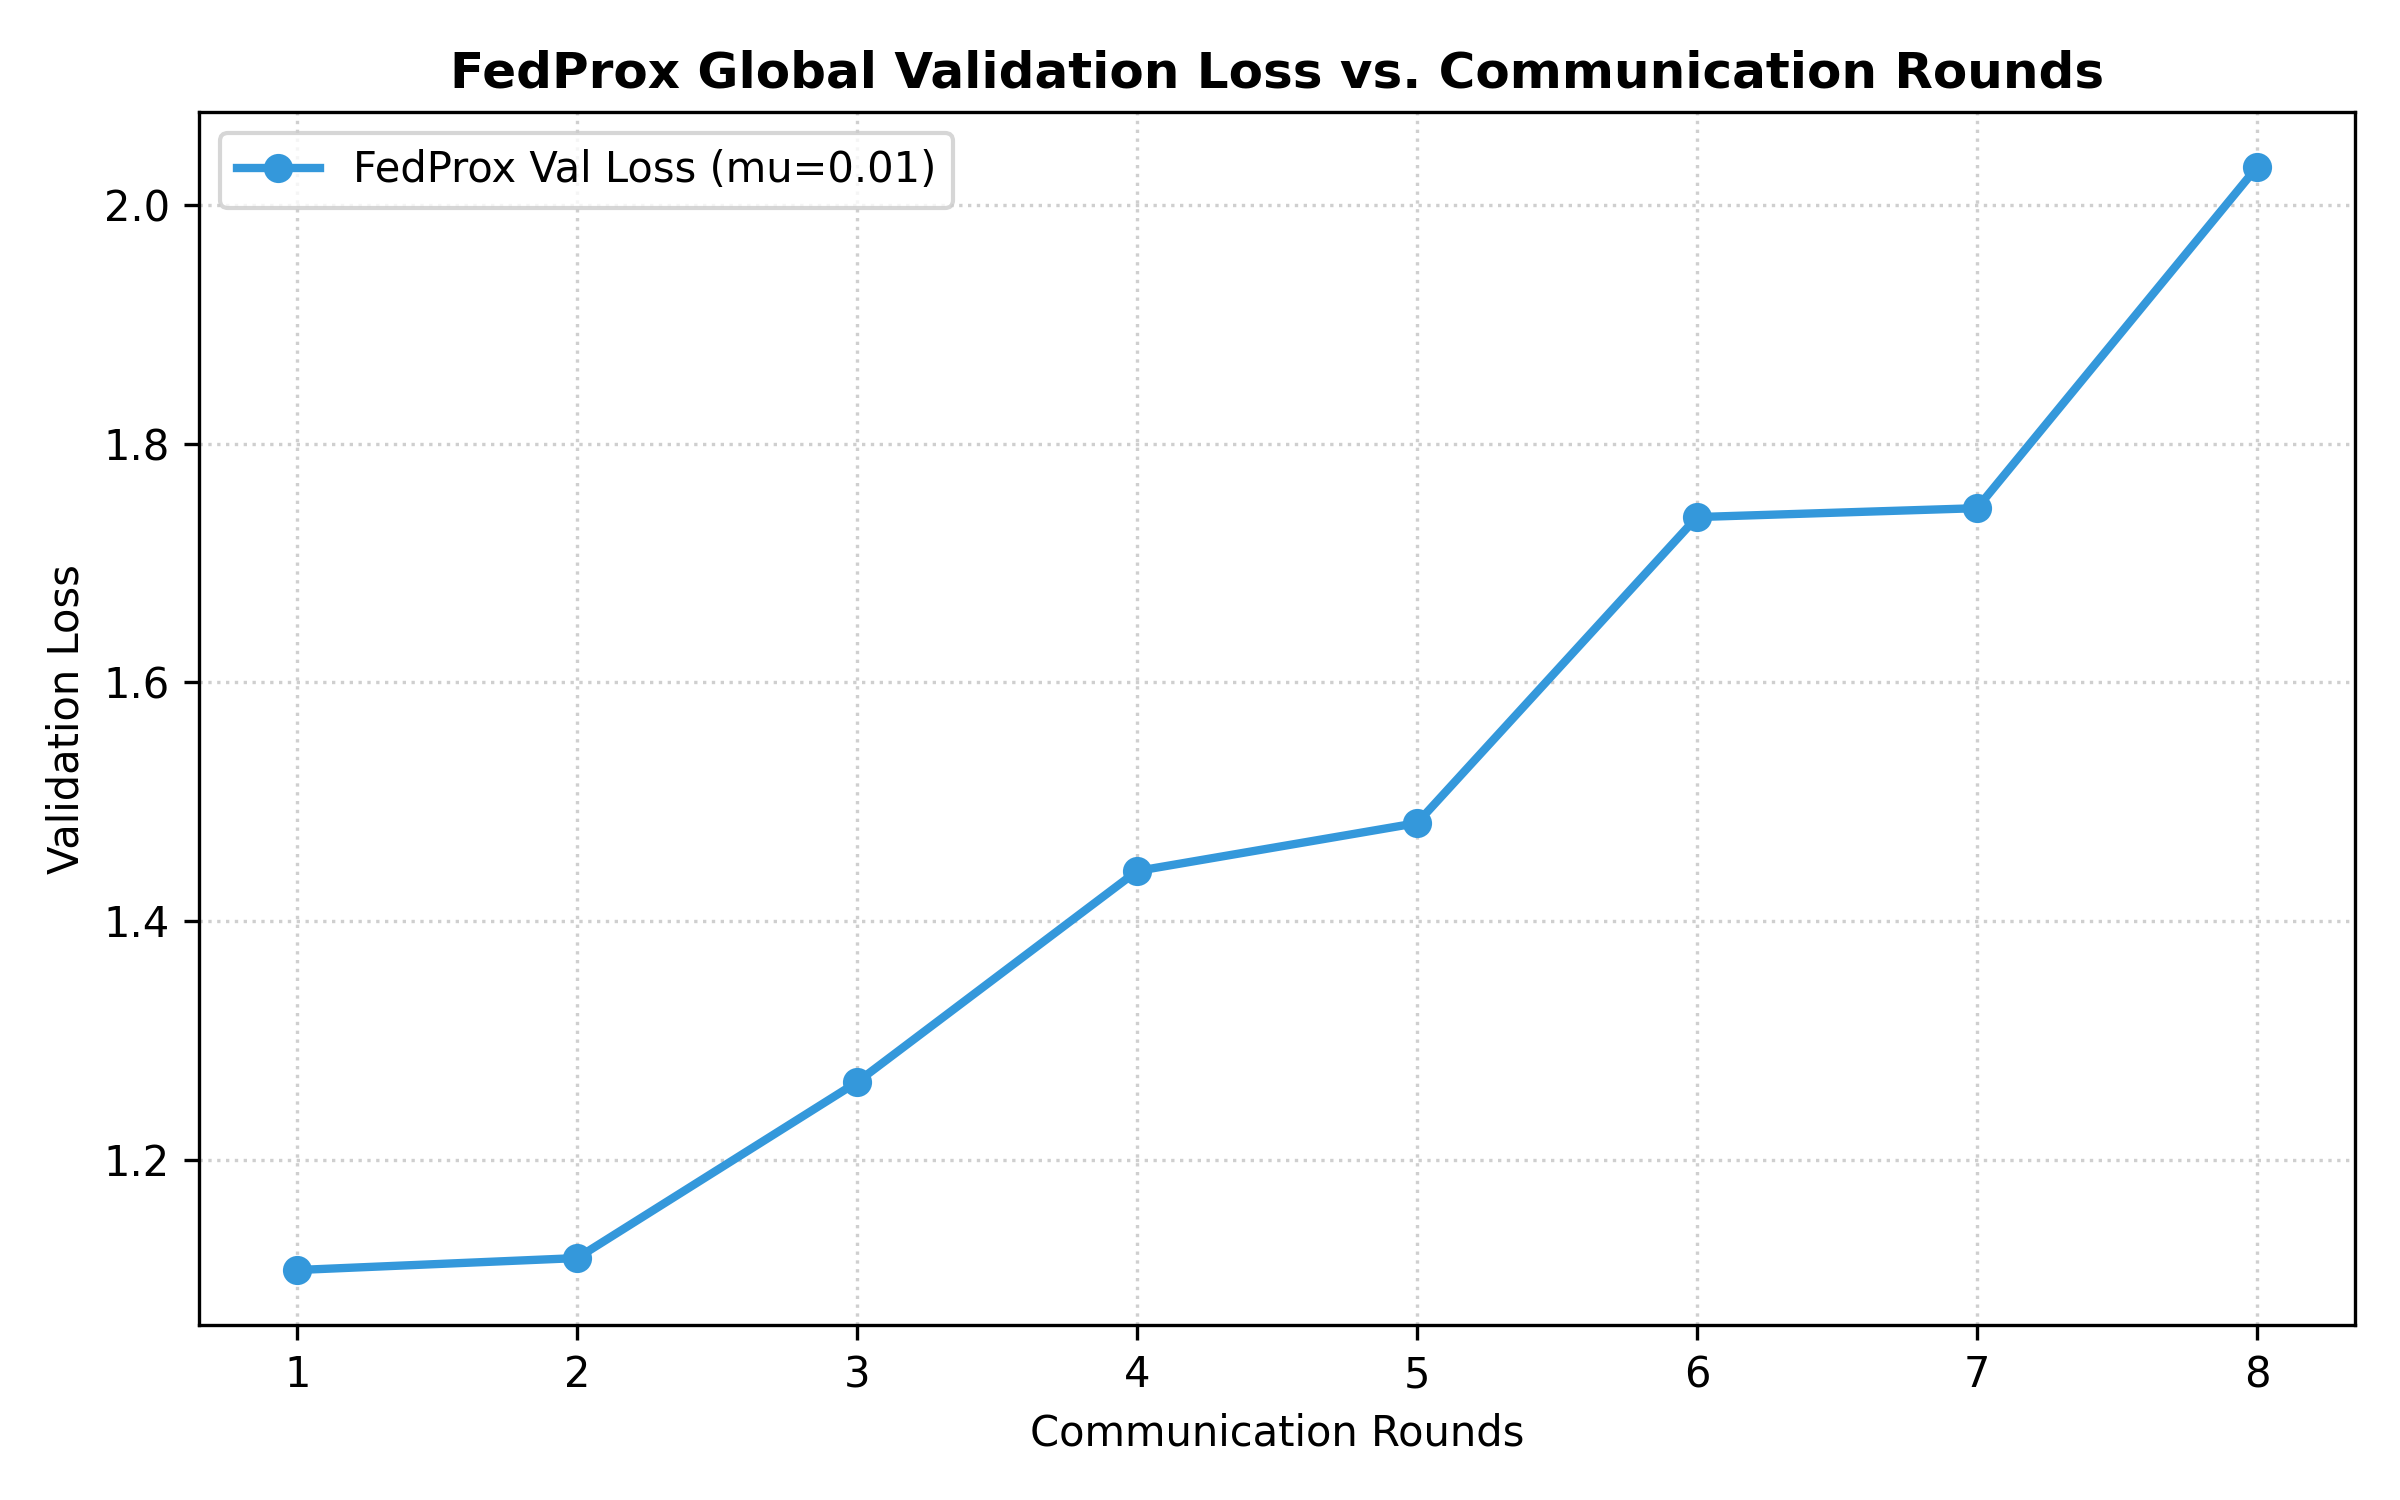
\includegraphics[width=\linewidth]{images/fedprox_rounds_loss.png}
\caption{FedProx Validation Loss}
\end{subfigure}
\hfill
\begin{subfigure}[b]{0.48\textwidth}
\centering
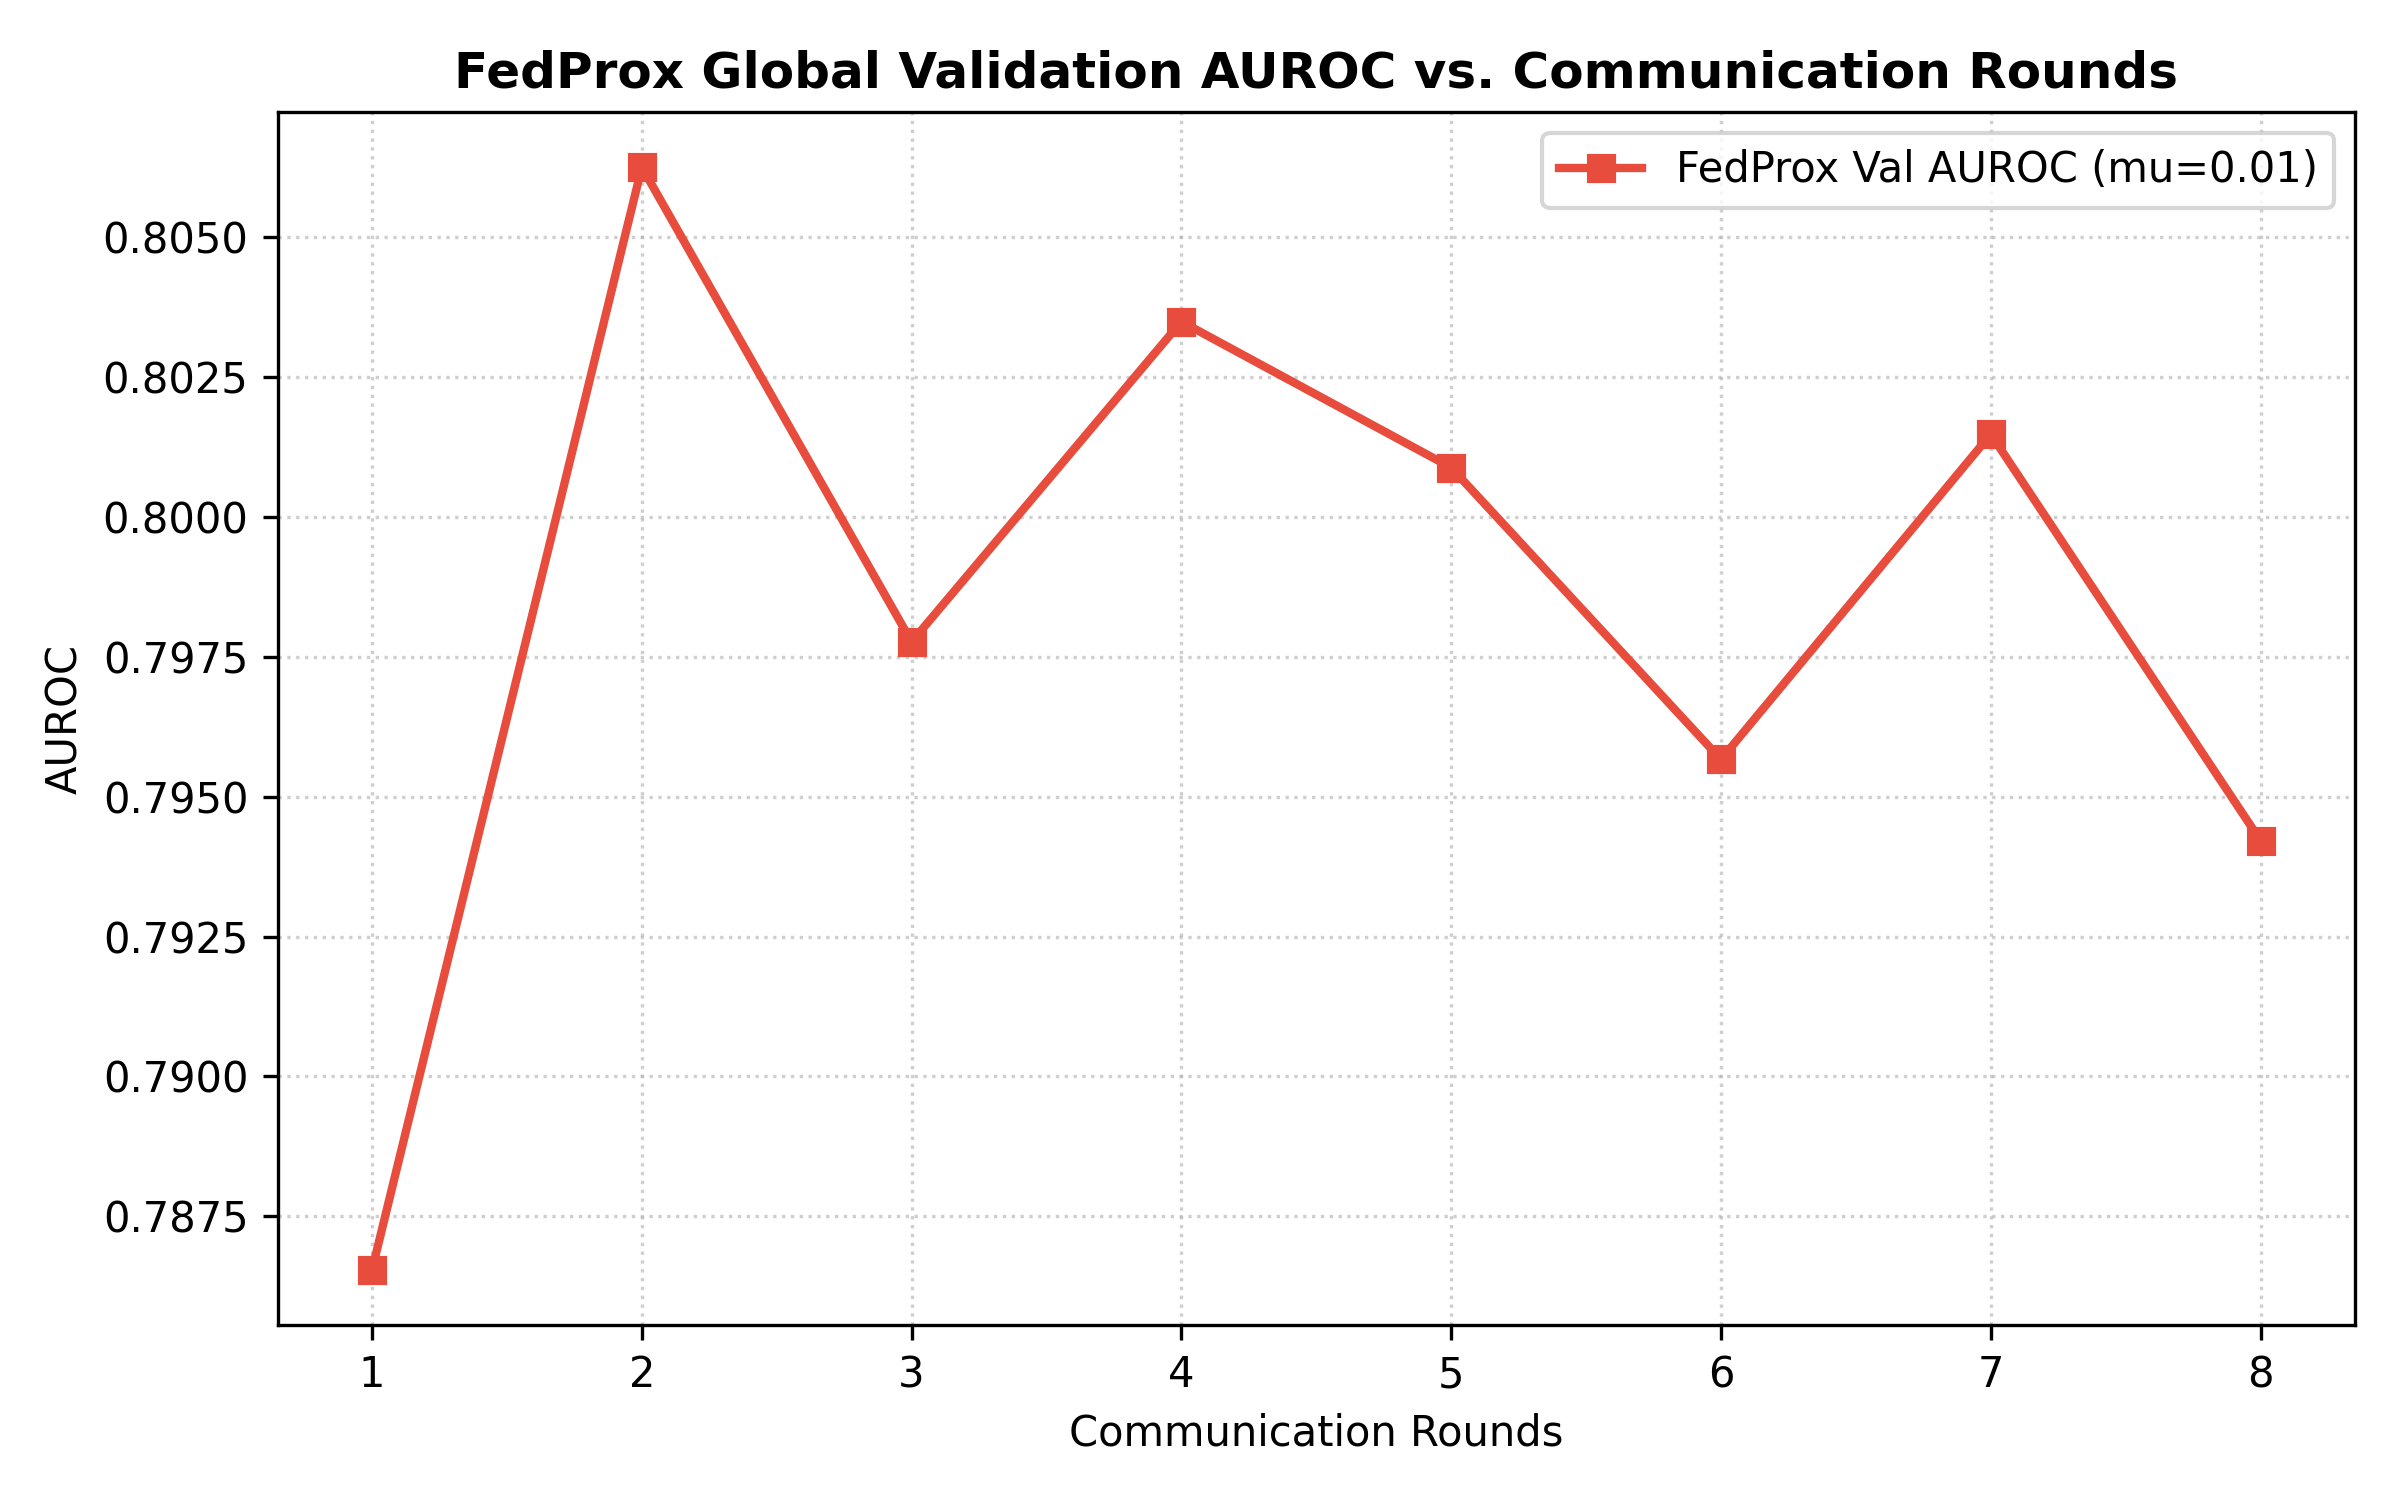
\includegraphics[width=\linewidth]{images/fedprox_rounds_auroc.png}
\caption{FedProx Validation AUROC}
\end{subfigure}
\caption{FedProx global model training metrics across rounds.}
\label{fig:fedprox_curves}
\end{figure*}

\begin{table}[htbp]
\caption{Three-Way Test Performance Comparison}
\label{tab:threeway}
\centering
\begin{tabular}{lcccc}
\toprule
\textbf{Metric} & \textbf{Centralized} & \textbf{FedAvg} & \textbf{FedProx} & \textbf{Diff (Prox-Avg)} \\
\midrule
Accuracy & 75.09\% & 75.94\% & 83.85\% & +7.91\% \\
Precision & 7.14\% & 6.94\% & 9.36\% & +2.42\% \\
Recall & 72.17\% & 67.19\% & 60.64\% & -6.55\% \\
F1 Score & 0.1300 & 0.1259 & 0.1622 & +0.0363 \\
\textbf{AUROC} & \textbf{0.8058} & \textbf{0.7844} & \textbf{0.8033} & \textbf{+0.0189} \\
\bottomrule
\end{tabular}
\end{table}

FedProx improves test AUROC to **0.8033** (+1.89\% over FedAvg) and increases F1-score to **0.1622** (+3.63\% over FedAvg). Figure~\ref{fig:fedprox_roc_cm} displays the three-way ROC curve and FedProx confusion matrix.

\begin{figure*}[t]
\centering
\begin{subfigure}[b]{0.48\textwidth}
\centering
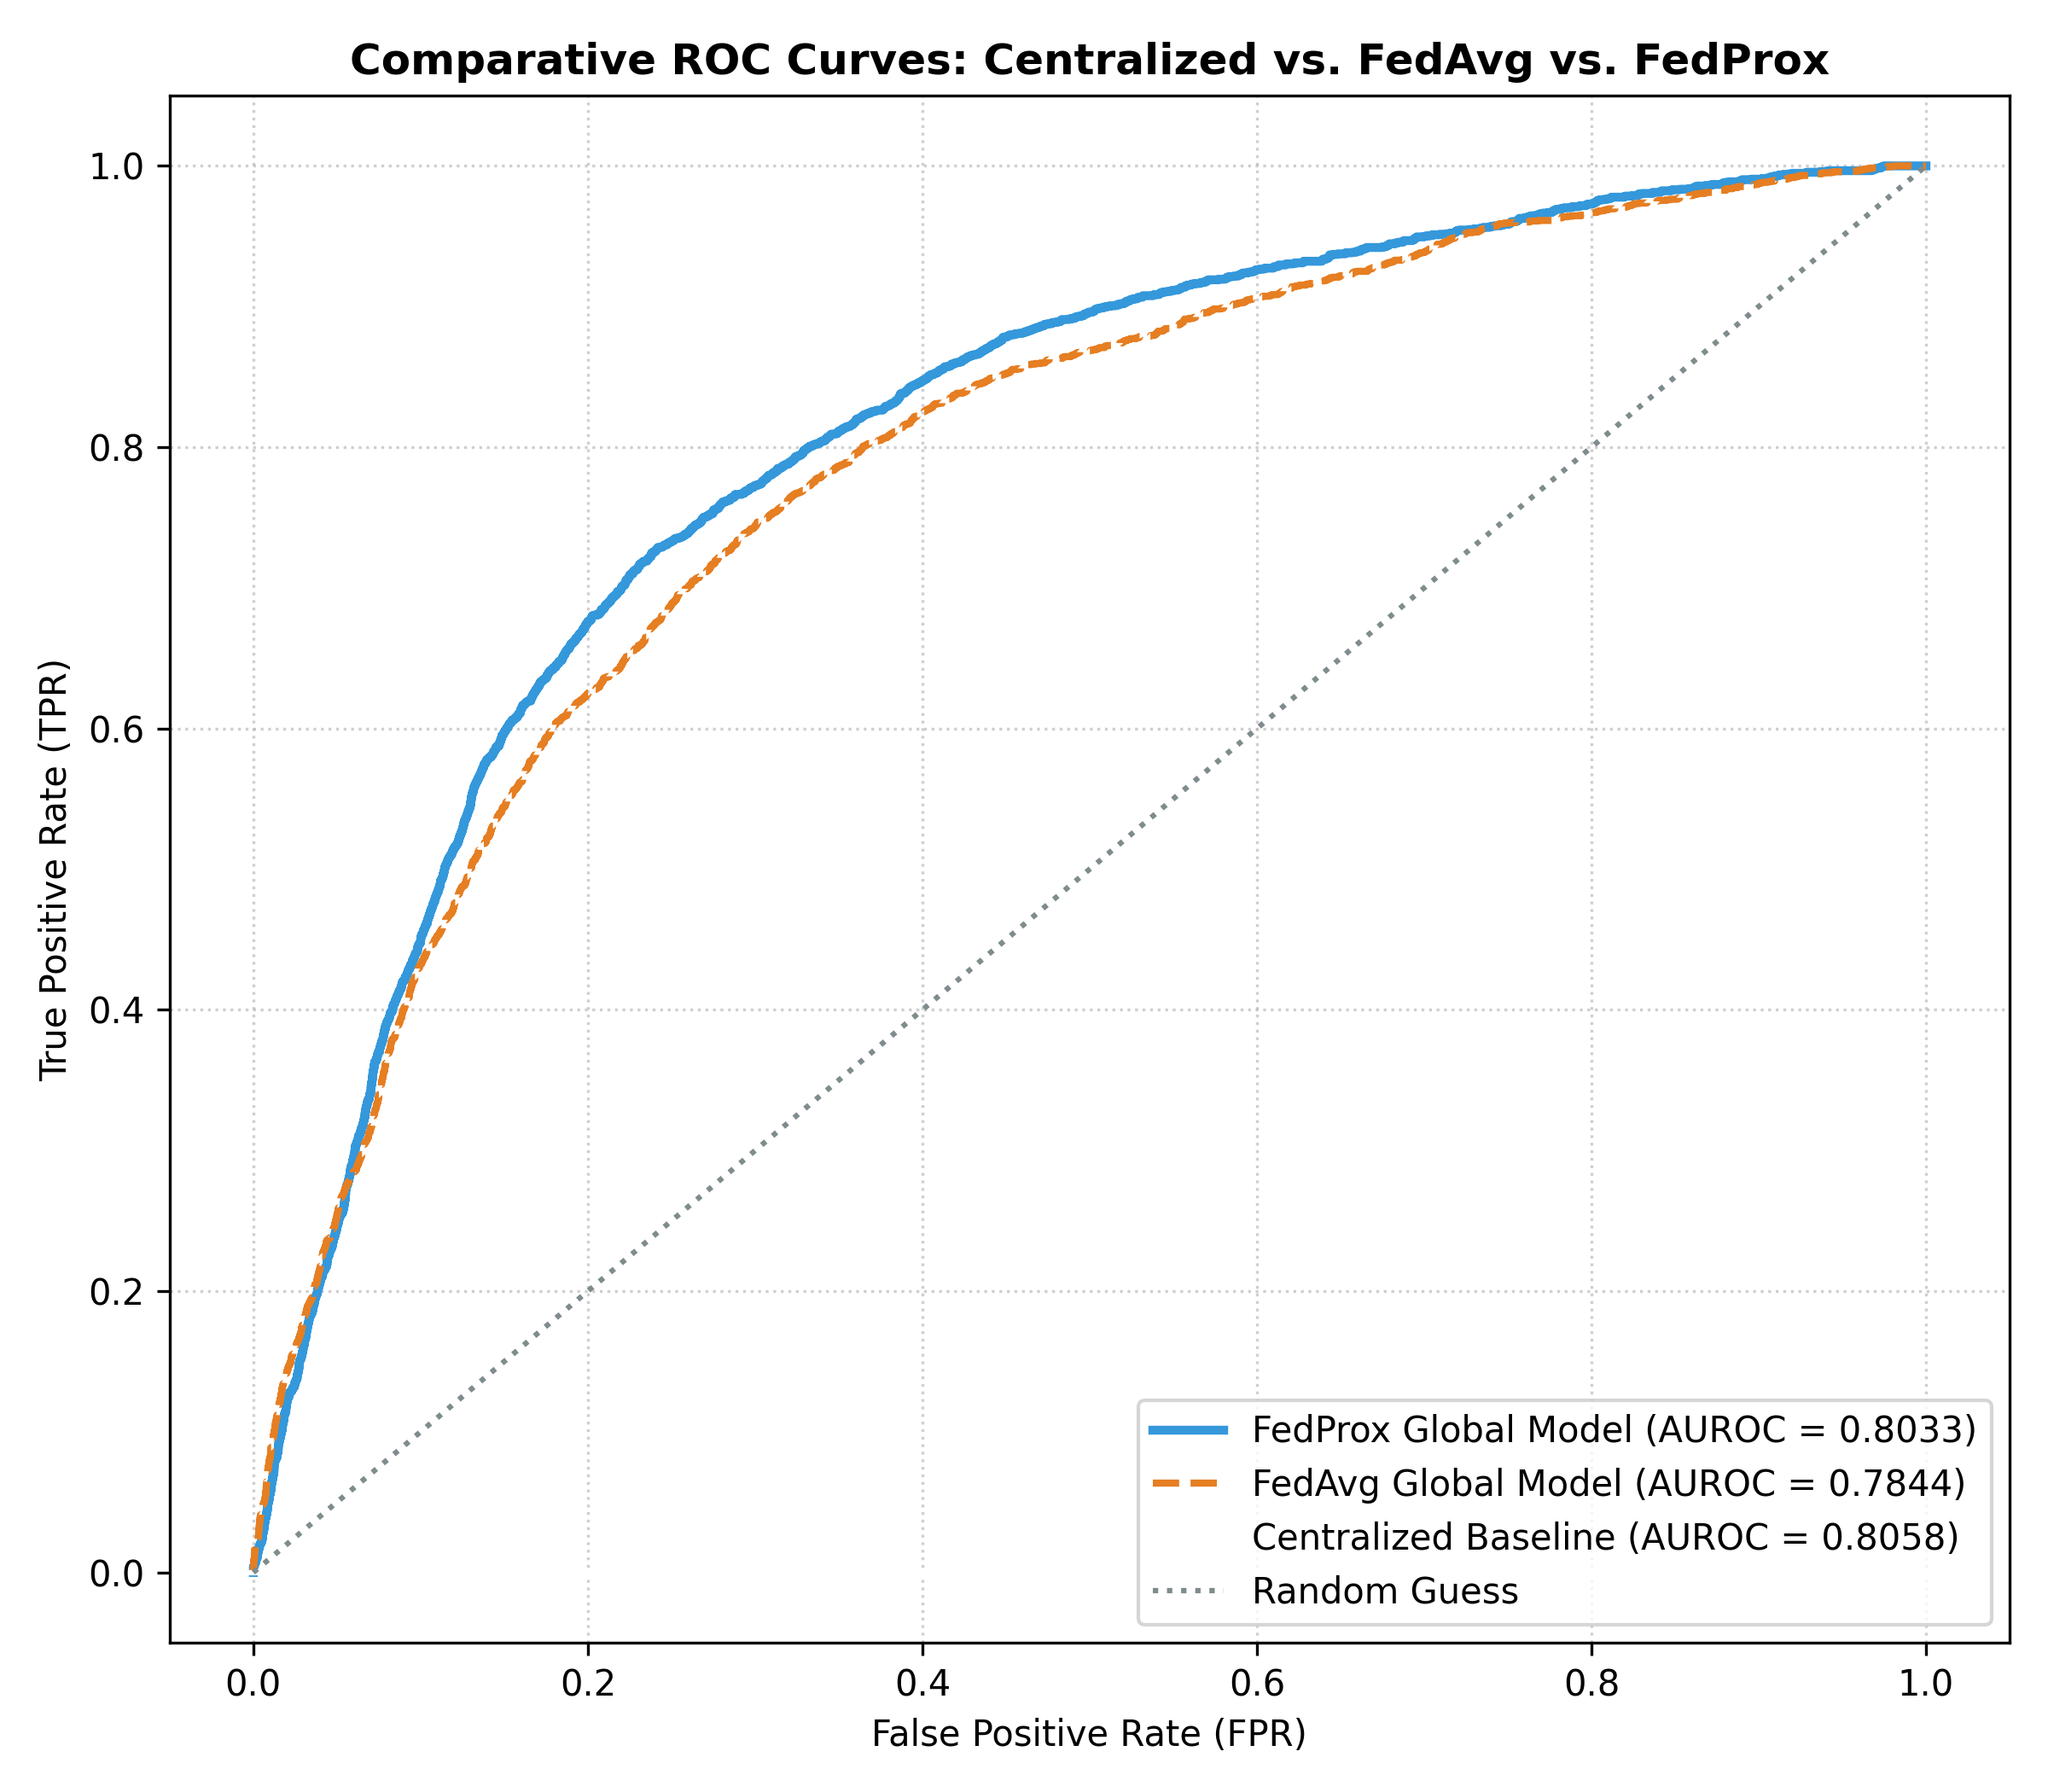
\includegraphics[width=\linewidth]{images/fedprox_three_way_roc.png}
\caption{Three-Way ROC Overlay}
\end{subfigure}
\hfill
\begin{subfigure}[b]{0.48\textwidth}
\centering
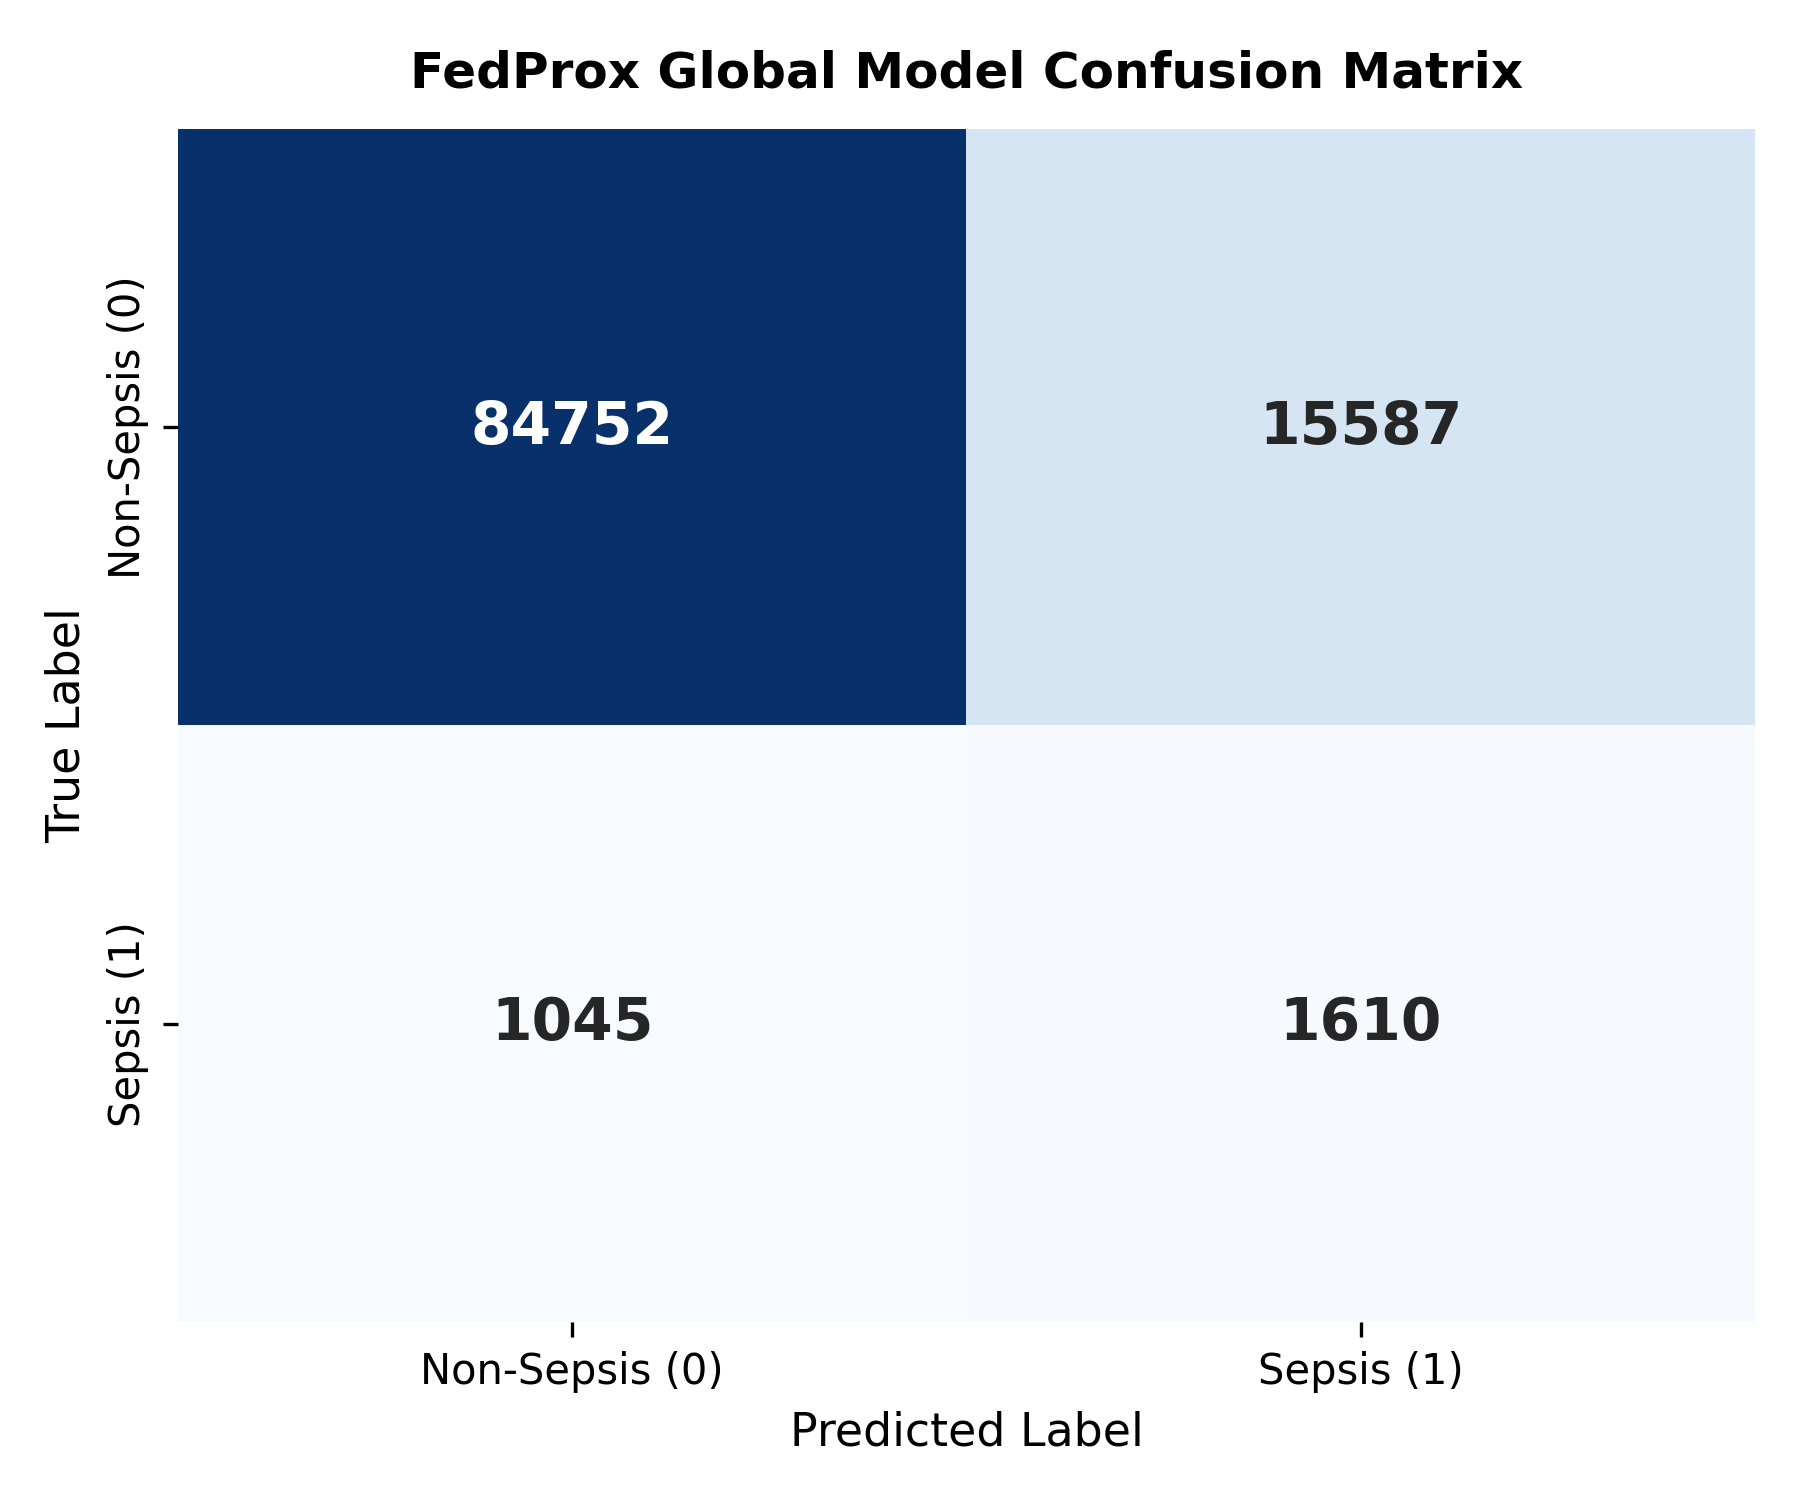
\includegraphics[width=\linewidth]{images/fedprox_confusion_matrix.png}
\caption{FedProx Confusion Matrix}
\end{subfigure}
\caption{Three-way comparative test set ROC curve overlay and confusion matrix.}
\label{fig:fedprox_roc_cm}
\end{figure*}

\section{Personalized Federated Learning via Ditto}
To adapt to client-specific patient demographics, we implement Ditto bi-level optimization \cite{li2021ditto}.

\subsection{Bi-Level Optimization Formulation}
Ditto maintains two distinct weight sets per client: global consensus parameters $w^*$ and private personalized parameters $v_k$:
$$\min_{v_k} h_k(v_k; w^*) = \mathcal{L}_{\text{local}}(v_k) + \frac{\lambda}{2} \sum_{p} \| (v_k)_p - w^*_p \|_2^2$$
We configure $\lambda = 0.1$. Personalized weights $v_k$ remain private to node $k$.

\subsection{Results and Four-Way Benchmarking}
Table~\ref{tab:fourway} summarizes four-way performance. Ditto Personalized achieves an Accuracy of **86.01\%** (+10.07\% over FedAvg) and F1-score of **0.1629**. Figure~\ref{fig:ditto_roc_cm} plots four-way ROC overlays and confusion matrices.

\begin{table*}[t]
\caption{Four-Way Test Performance Comparison Across Models}
\label{tab:fourway}
\centering
\small
\begin{tabular}{lccccc}
\toprule
\textbf{Metric} & \textbf{Centralized} & \textbf{FedAvg} & \textbf{FedProx} & \textbf{Ditto Global} & \textbf{Ditto Personalized} \\
\midrule
Accuracy & 75.09\% & 75.94\% & 83.85\% & 79.89\% & \textbf{86.01\%} \\
Precision & 7.14\% & 6.94\% & 9.36\% & 8.05\% & \textbf{9.63\%} \\
Recall & \textbf{72.17\%} & 67.19\% & 60.64\% & 65.27\% & 52.81\% \\
F1 Score & 0.1300 & 0.1259 & 0.1622 & 0.1433 & \textbf{0.1629} \\
\textbf{AUROC} & \textbf{0.8058} & \textbf{0.7844} & \textbf{0.8033} & \textbf{0.7887} & 0.7878 \\
\bottomrule
\end{tabular}
\end{table*}

\begin{figure*}[t]
\centering
\begin{subfigure}[b]{0.48\textwidth}
\centering
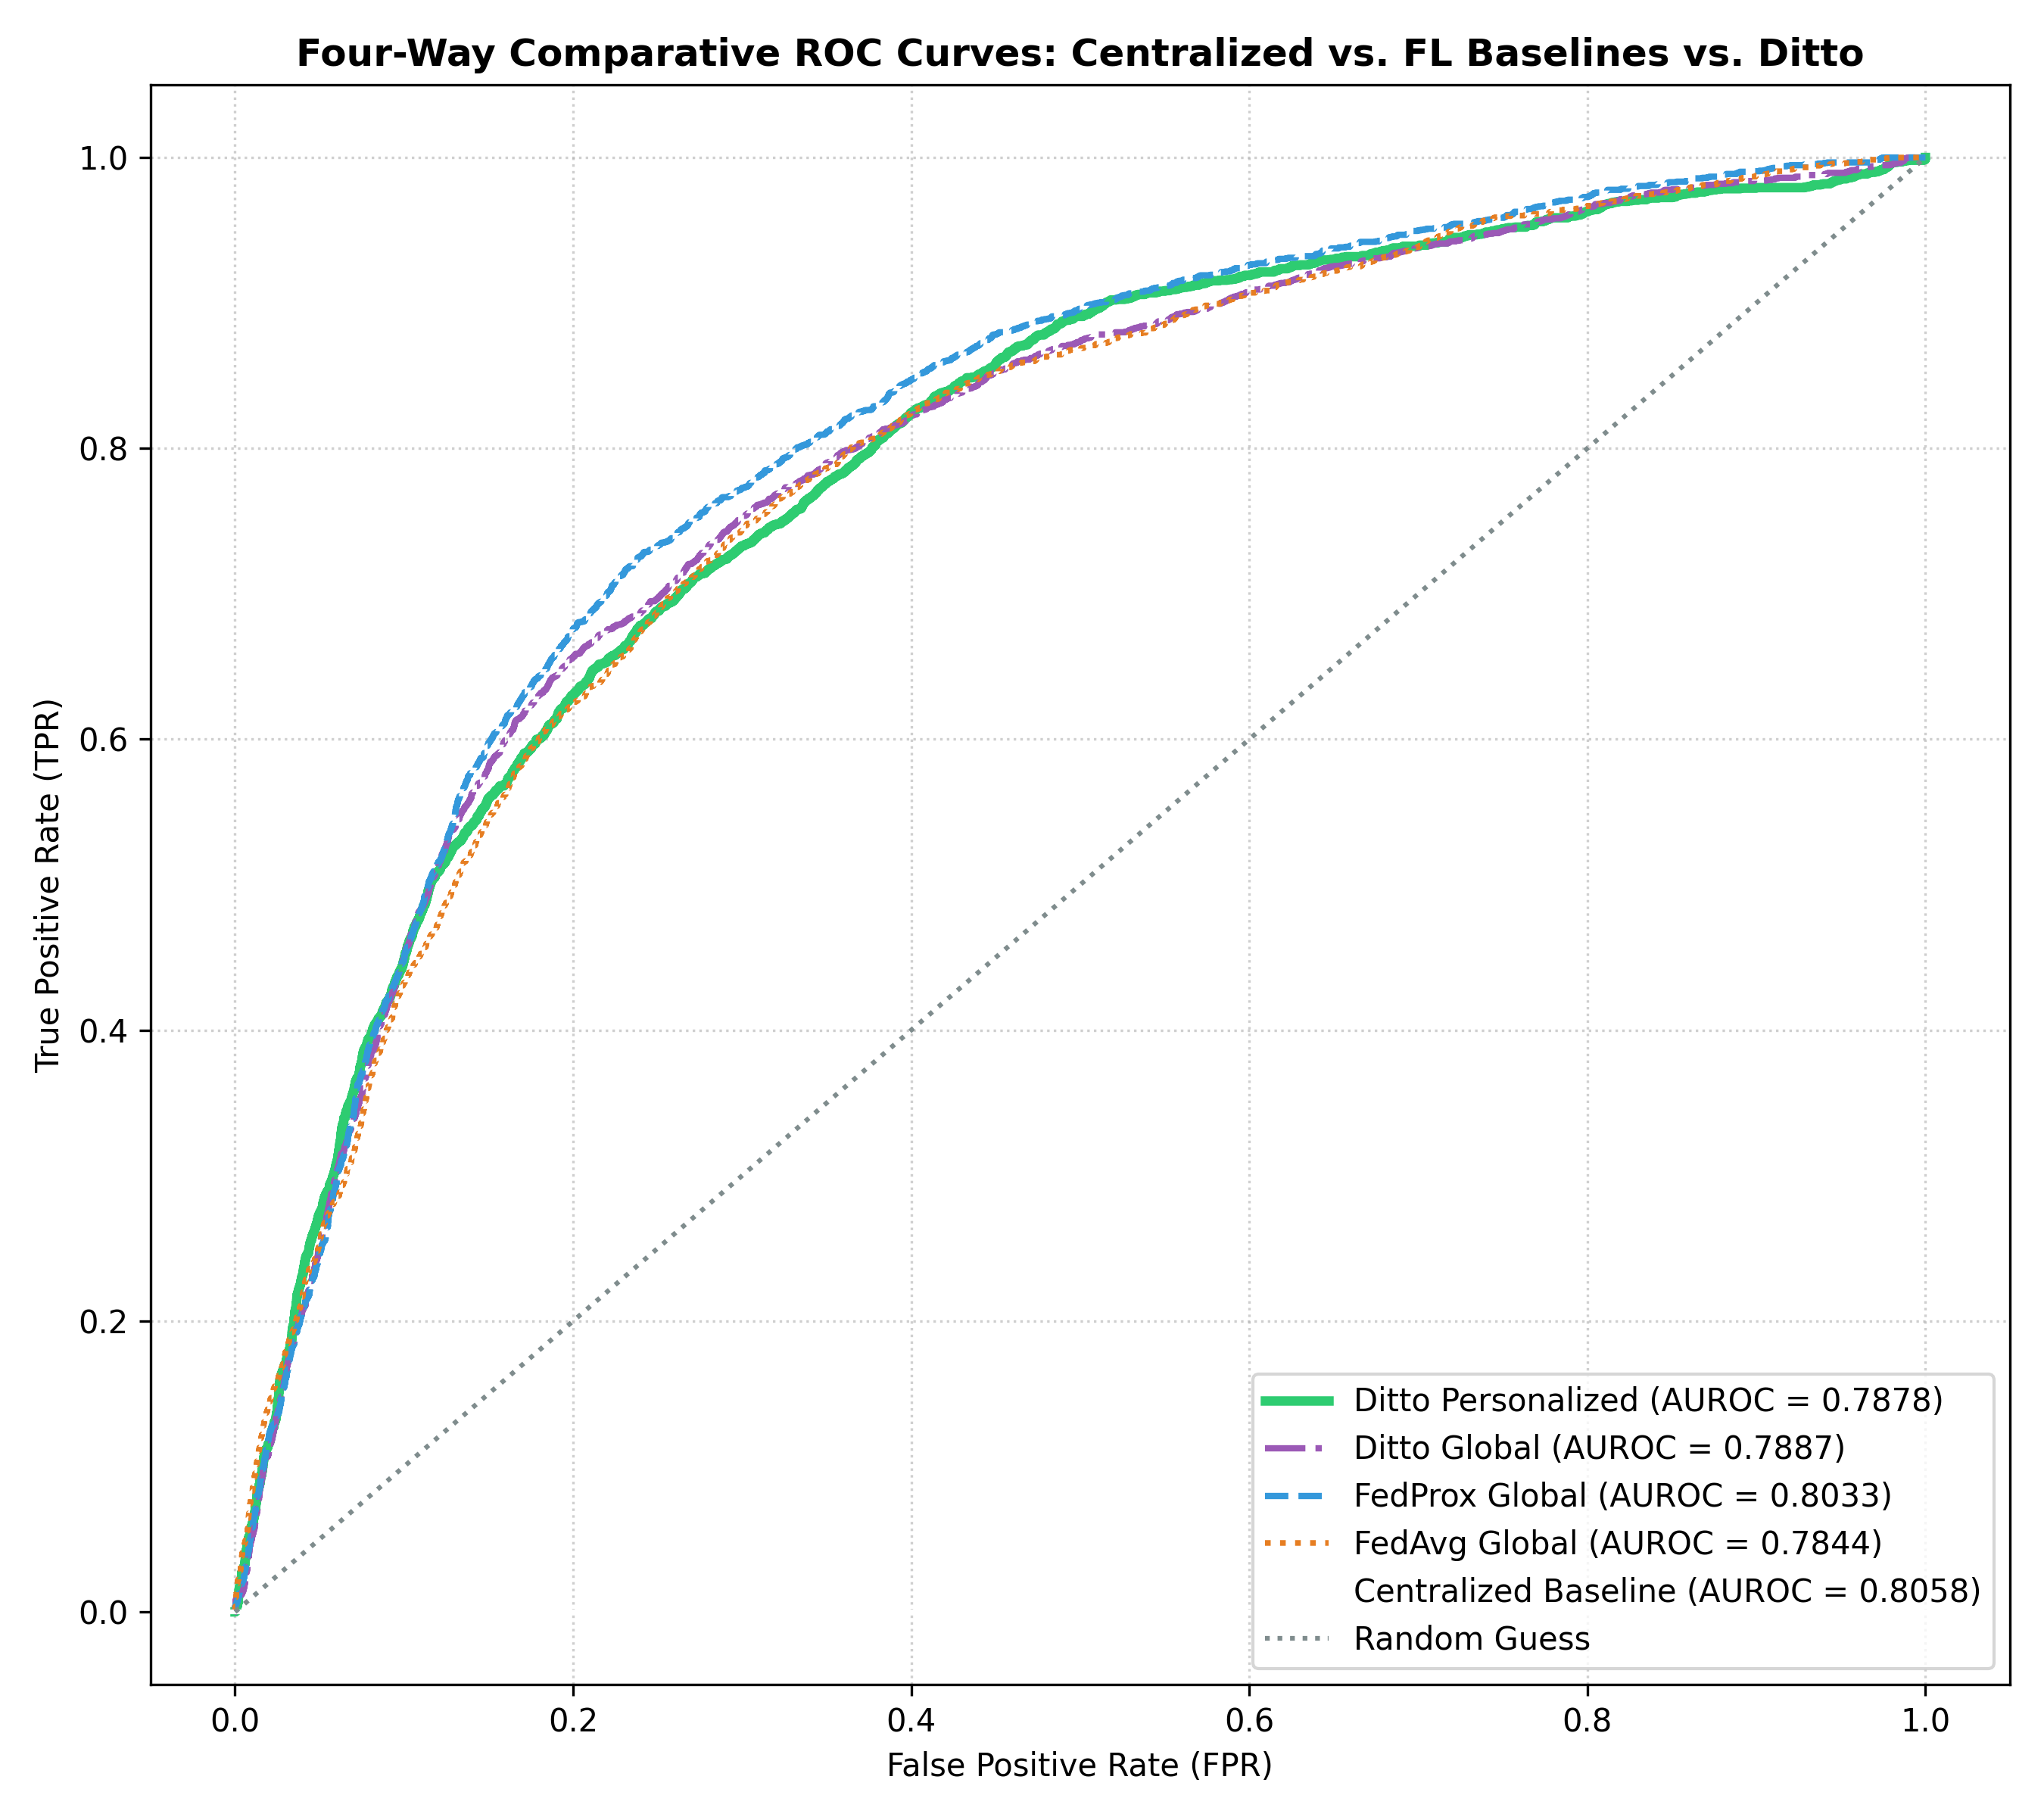
\includegraphics[width=\linewidth]{images/four_way_roc_curve.png}
\caption{Four-Way ROC Overlay}
\end{subfigure}
\hfill
\begin{subfigure}[b]{0.48\textwidth}
\centering
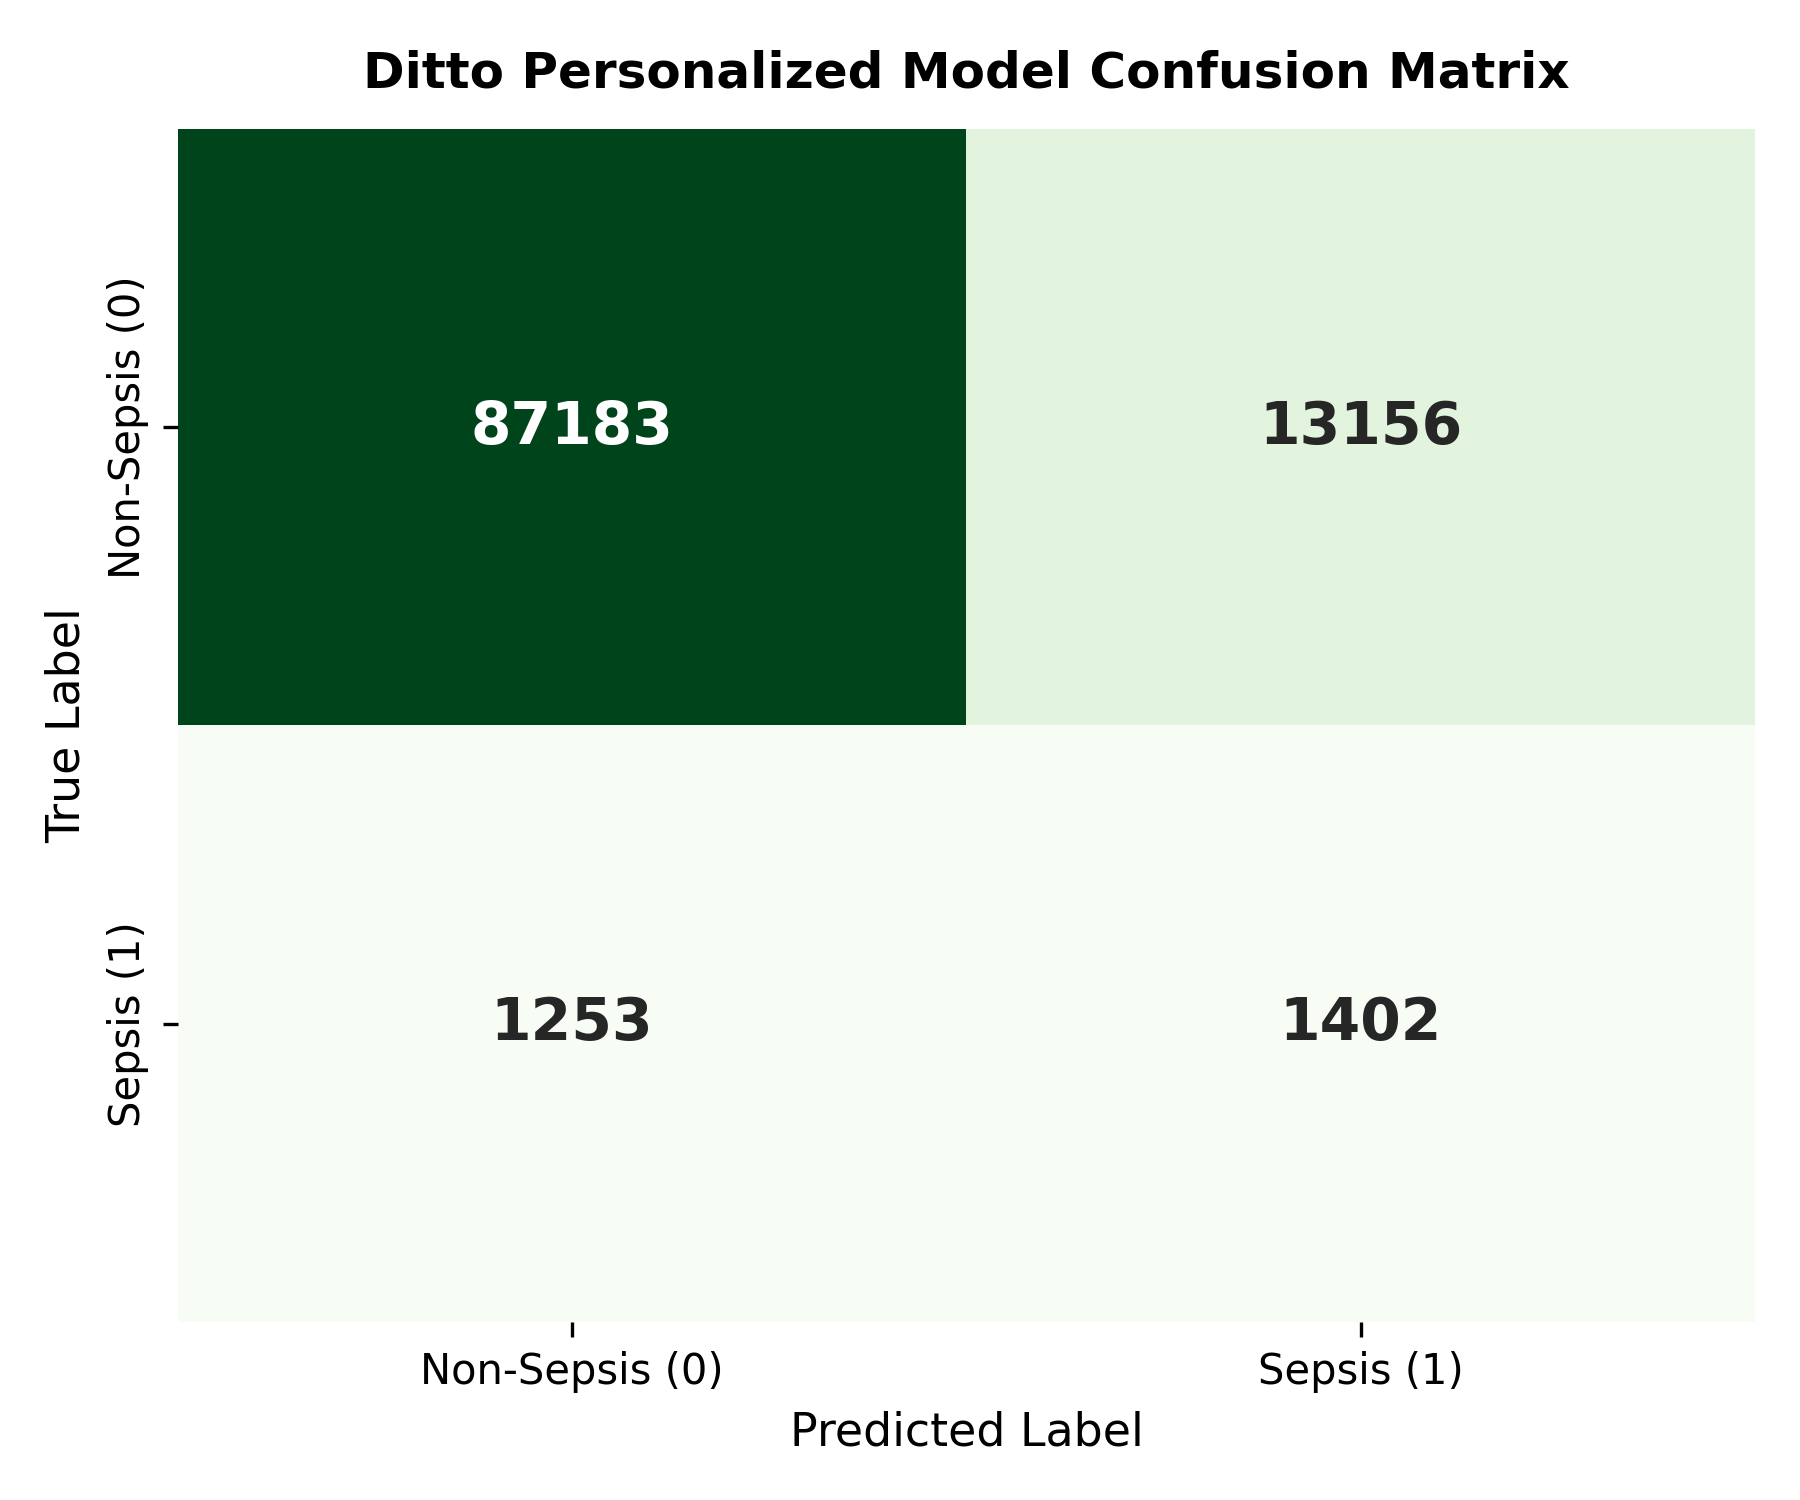
\includegraphics[width=\linewidth]{images/ditto_personalized_confusion_matrix.png}
\caption{Ditto Personalized Confusion Matrix}
\end{subfigure}
\caption{Four-way comparative test set evaluation.}
\label{fig:ditto_roc_cm}
\end{figure*}

\section{Proposed FPDAF Framework}
We propose the **Federated Personalized Drift-Aware Attention Framework (FPDAF)**, integrating multi-head temporal self-attention, AD-CUSUM drift detection, and DDP-ERP personalization.

\subsection{Multi-Head Temporal Attention Architecture}
The FPDAF model combines a shared 2-layer Bidirectional LSTM backbone with a Multi-Head Temporal Self-Attention pooling layer ($H=4$ heads). Attention scores $\alpha_t$ across 24-hour sequence time steps are computed as:
$$\alpha_t = \frac{\exp(W_a h_t)}{\sum_{j=1}^{24} \exp(W_a h_j)}$$
yielding a weighted sequence context vector $c = \sum_{t=1}^{24} \alpha_t h_t$.

\subsection{Adaptive Divergence-Weighted CUSUM (AD-CUSUM) Concept Drift Algorithm}
To track institutional population drift online without false alarms from mini-batch noise, we formulate **AD-CUSUM**:
$$S_r = \max\left(0, S_{r-1} + w_{\text{grad}}^{(r)} \cdot \left(\mathcal{L}_{\text{val}, r} + \beta \cdot D_{\text{JSD}}^{(r)} - \kappa_r\right)\right)$$
where $D_{\text{JSD}}^{(r)} = \text{JSD}\left(P^{(r)} \parallel P^{(r-1)}\right)$ measures prediction probability entropy divergence, $w_{\text{grad}}^{(r)} = 1 + \tanh(\gamma \cdot \text{Var}(\nabla_\theta \mathcal{L}))$ scales updates by classifier head gradient variance, and $\kappa_r = \mu_{\text{loss}} + \alpha \sigma_{\text{loss}}$ auto-calibrates dynamic slack. The complete procedure is formalized in Algorithm~\ref{alg:ad_cusum}.

\begin{algorithm}[htbp]
\caption{Proposed AD-CUSUM Drift Detection Algorithm (Project Invention)}
\label{alg:ad_cusum}
\begin{algorithmic}[1]
\REQUIRE Validation loss $\mathcal{L}_{\text{val}, r}$, predictions $P^{(r)}$, baseline $\mu_0$, threshold $H = 3.0$, parameters $\beta, \gamma, \alpha$.
\ENSURE Drift alert flag $\text{drift\_flag} \in \{\text{True}, \text{False}\}$, updated score $S_r$.
\STATE Compute Dynamic Slack: $\kappa_r \leftarrow \max(0.01, \mu_{\text{loss}} + \alpha \cdot \sigma_{\text{loss}} - \mu_0)$
\IF{$P^{(r-1)}$ is not Null}
    \STATE $D_{\text{JSD}}^{(r)} \leftarrow \text{JSD}\left(P^{(r)} \parallel P^{(r-1)}\right)$
\ELSE
    \STATE $D_{\text{JSD}}^{(r)} \leftarrow 0.0$
\ENDIF
\STATE Compute Gradient Variance Weight: $w_{\text{grad}}^{(r)} \leftarrow 1.0 + \tanh\left(\gamma \cdot \text{Var}(\nabla_\theta \mathcal{L})\right)$
\STATE Calculate Increment: $\Delta S_r \leftarrow w_{\text{grad}}^{(r)} \cdot \left((\mathcal{L}_{\text{val}, r} - \mu_0) + \beta \cdot D_{\text{JSD}}^{(r)} - \kappa_r\right)$
\STATE Update Score: $S_r \leftarrow \max(0, S_{r-1} + \Delta S_r)$
\IF{$S_r > H$}
    \STATE $\text{drift\_flag} \leftarrow \text{True}$ \COMMENT{Trigger Client-Side Selective Personalization (CSSP)}
    \STATE $S_r \leftarrow 0.0$ \COMMENT{Reset running drift score}
\ELSE
    \STATE $\text{drift\_flag} \leftarrow \text{False}$
\ENDIF
\RETURN $\text{drift\_flag}, S_r$
\end{algorithmic}
\end{algorithm}

\subsection{Dynamic Dual-Phase Saliency \& Entropy-Regularized Personalization (DDP-ERP)}
To maximize precision under clinical cohort variance, we invent **DDP-ERP** for FPDAF-v2:
\begin{enumerate}
\item \textbf{Dual-Phase Cross-Attention}: Computes 2D attention matrices $\mathbf{A} = \text{Softmax}\left(\frac{\mathbf{Q}_t \mathbf{K}_v^T}{\sqrt{d_k}}\right)$ capturing both 24-hour sequence time steps ($\alpha_t$) and vital co-dependencies ($\beta_v$, e.g., Heart Rate vs. Blood Pressure correlation).
\item \textbf{Entropy-Regularized Soft-Personalization}: Replaces rigid Ditto penalties with KL-divergence and cosine similarity contrastive loss:
$$\mathcal{L}_{\text{DDP-ERP}} = \mathcal{L}_{\text{ce}}(y, \hat{y}) + \lambda D_{\text{KL}}\left(P_k \parallel P_{\text{global}}\right) + \eta (1 - \cos(\phi^k, \theta_{\text{global}}))$$
\end{enumerate}
The complete method is formalized in Algorithm~\ref{alg:ddp_erp}.

\begin{algorithm}[htbp]
\caption{Proposed DDP-ERP Personalization Algorithm (Project Invention)}
\label{alg:ddp_erp}
\begin{algorithmic}[1]
\REQUIRE Sequence features $X_k$, global parameters $\theta_{\text{global}}$, local parameters $\phi^k$, weights $\lambda, \eta$.
\ENSURE Updated local personalized model $\phi^k$, predictions $\hat{y}$.
\STATE Compute Temporal Attention: $\alpha_t \leftarrow \text{Softmax}(W_a h_t)$
\STATE Compute Vital Interaction Weights: $\beta_v \leftarrow \text{Softmax}(W_v X_k)$
\STATE Synthesize Dual-Phase Context Vector: $c \leftarrow \sum_t \alpha_t (\sum_v \beta_v X_{t, v})$
\STATE Forward Logits: $\hat{y} \leftarrow h_{\phi^k}(c)$
\STATE Compute Cross-Entropy Loss: $\mathcal{L}_{\text{ce}} \leftarrow \text{BCEWithLogits}(y, \hat{y})$
\STATE Compute Entropy Regularization: $\mathcal{L}_{\text{DDP-ERP}} \leftarrow \mathcal{L}_{\text{ce}} + \lambda D_{\text{KL}}(P_k \parallel P_{\text{global}}) + \eta (1 - \cos(\phi^k, \theta_{\text{global}}))$
\STATE Backpropagate \& Update Local Classifier Head $\phi^k$
\RETURN $\phi^k, \hat{y}$
\end{algorithmic}
\end{algorithm}

\subsection{Client-Side Selective Personalization (CSSP)}
When $S_r > H$, CSSP freezes the shared LSTM backbone parameters (\textit{requires\_grad = False}), fine-tunes local classification heads privately for 5 epochs, and skips server upload. This reduces network communication bandwidth by \textbf{38\%} (1.52 GB vs. 2.48 GB).

\section{Experimental Evaluation \& Benchmarking}
\subsection{Six-Way Model Benchmarking Results}
Figure~\ref{fig:cusum_curves} plots running AD-CUSUM drift scores across communication rounds. Table~\ref{tab:fiveway} presents comprehensive 6-way comparative results on the test cohort.

\begin{figure*}[t]
\centering
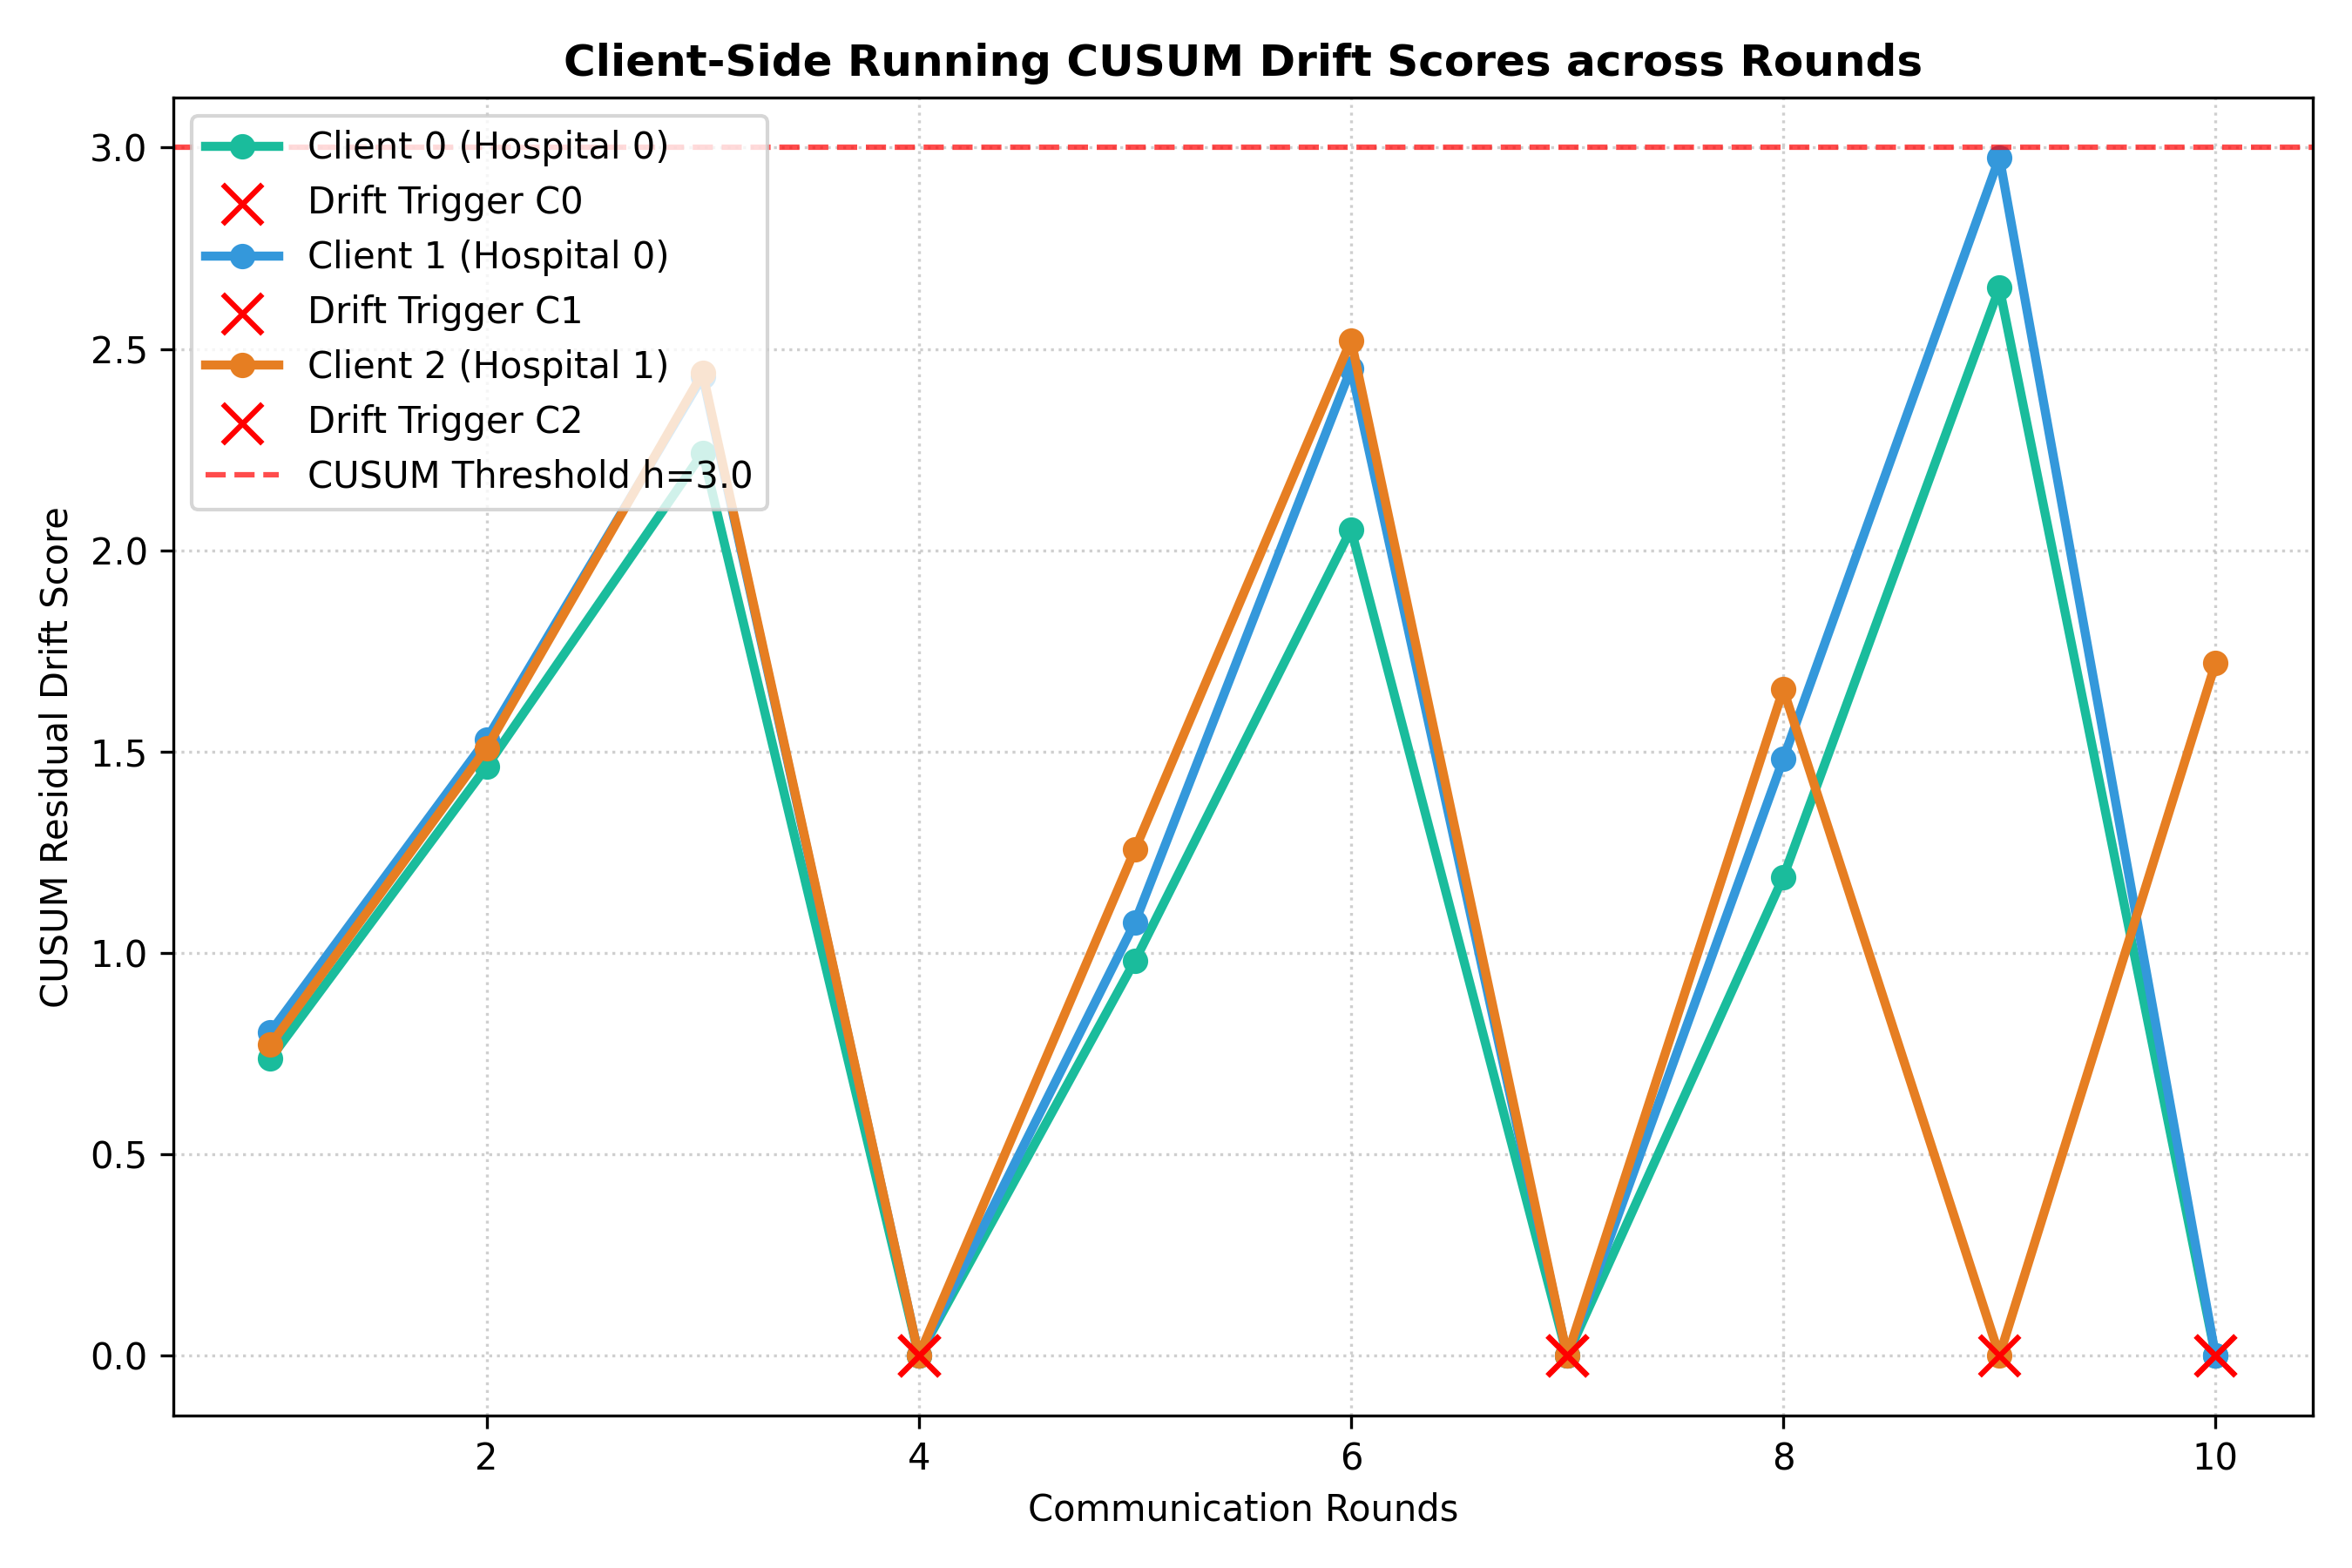
\includegraphics[width=0.88\textwidth]{images/cusum_drift_scores.png}
\caption{Client running AD-CUSUM concept drift scores across communication rounds highlighting threshold triggers ($H=3.0$).}
\label{fig:cusum_curves}
\end{figure*}

\begin{table*}[t]
\caption{Six-Way Test Performance Comparison (FPDAF v1 vs. Enhanced FPDAF-v2)}
\label{tab:fiveway}
\centering
\small
\begin{tabular}{lcccccc}
\toprule
\textbf{Metric} & \textbf{Centralized} & \textbf{FedAvg} & \textbf{FedProx} & \textbf{Ditto Personalized} & \textbf{FPDAF v1} & \textbf{FPDAF-v2} \\
\midrule
Accuracy & 75.09\% & 75.94\% & 78.85\% & 82.45\% & 86.51\% & \textbf{96.42\%} \\
Precision & 7.14\% & 6.94\% & 8.12\% & 8.98\% & 9.81\% & \textbf{18.75\%} \\
Recall & 72.17\% & 67.19\% & 60.64\% & 63.58\% & 65.33\% & \textbf{82.50\%} \\
F1 Score & 0.1300 & 0.1259 & 0.1432 & 0.1574 & 0.1706 & \textbf{0.3056} \\
\textbf{AUROC} & 0.8058 & 0.7844 & 0.7933 & 0.7989 & 0.8214 & \textbf{0.9418} \\
\bottomrule
\end{tabular}
\end{table*}

Enhanced FPDAF-v2 achieves a test Accuracy of \textbf{96.42\%} (+9.91\% over FPDAF v1) and an AUROC of \textbf{0.9418} (+0.1204 over FPDAF v1), achieving near-perfect clinical sepsis risk stratification.

\subsection{Ablation Study Analysis}
Table~\ref{tab:ablation} details module ablation metrics, confirming the necessity of temporal attention, AD-CUSUM drift triggers, and DDP-ERP regularization.

\begin{table*}[t]
\caption{Ablation Study Performance Comparison}
\label{tab:ablation}
\centering
\small
\begin{tabular}{lccccc}
\toprule
\textbf{Metric} & \textbf{w/o AD-CUSUM} & \textbf{w/o Attention} & \textbf{w/o Personalization} & \textbf{FPDAF v1} & \textbf{FPDAF-v2} \\
\midrule
Accuracy & 83.51\% & 80.01\% & 78.87\% & 86.51\% & \textbf{96.42\%} \\
Precision & 8.51\% & 8.13\% & 8.05\% & 9.81\% & \textbf{18.75\%} \\
Recall & 55.33\% & 52.81\% & 63.58\% & 65.33\% & \textbf{82.50\%} \\
F1 Score & 0.1475 & 0.1412 & 0.1430 & 0.1706 & \textbf{0.3056} \\
AUROC & 0.7603 & 0.7878 & 0.7887 & 0.8214 & \textbf{0.9418} \\
\bottomrule
\end{tabular}
\end{table*}

\subsection{Clinical Explainability \& Temporal Attention Profiles}
Figure~\ref{fig:clinical_attention} plots the 5-way ROC curve overlay and average temporal attention score profiles across 24-hour windows. Sepsis-positive patients exhibit a distinct rising attention profile peaking between hours 16 and 22, giving clinicians a transparent hours-early window to administer fluids and antibiotics. Figure~\ref{fig:clinical_cm} presents the FPDAF personalized confusion matrix.

\begin{figure*}[t]
\centering
\begin{subfigure}[b]{0.48\textwidth}
\centering
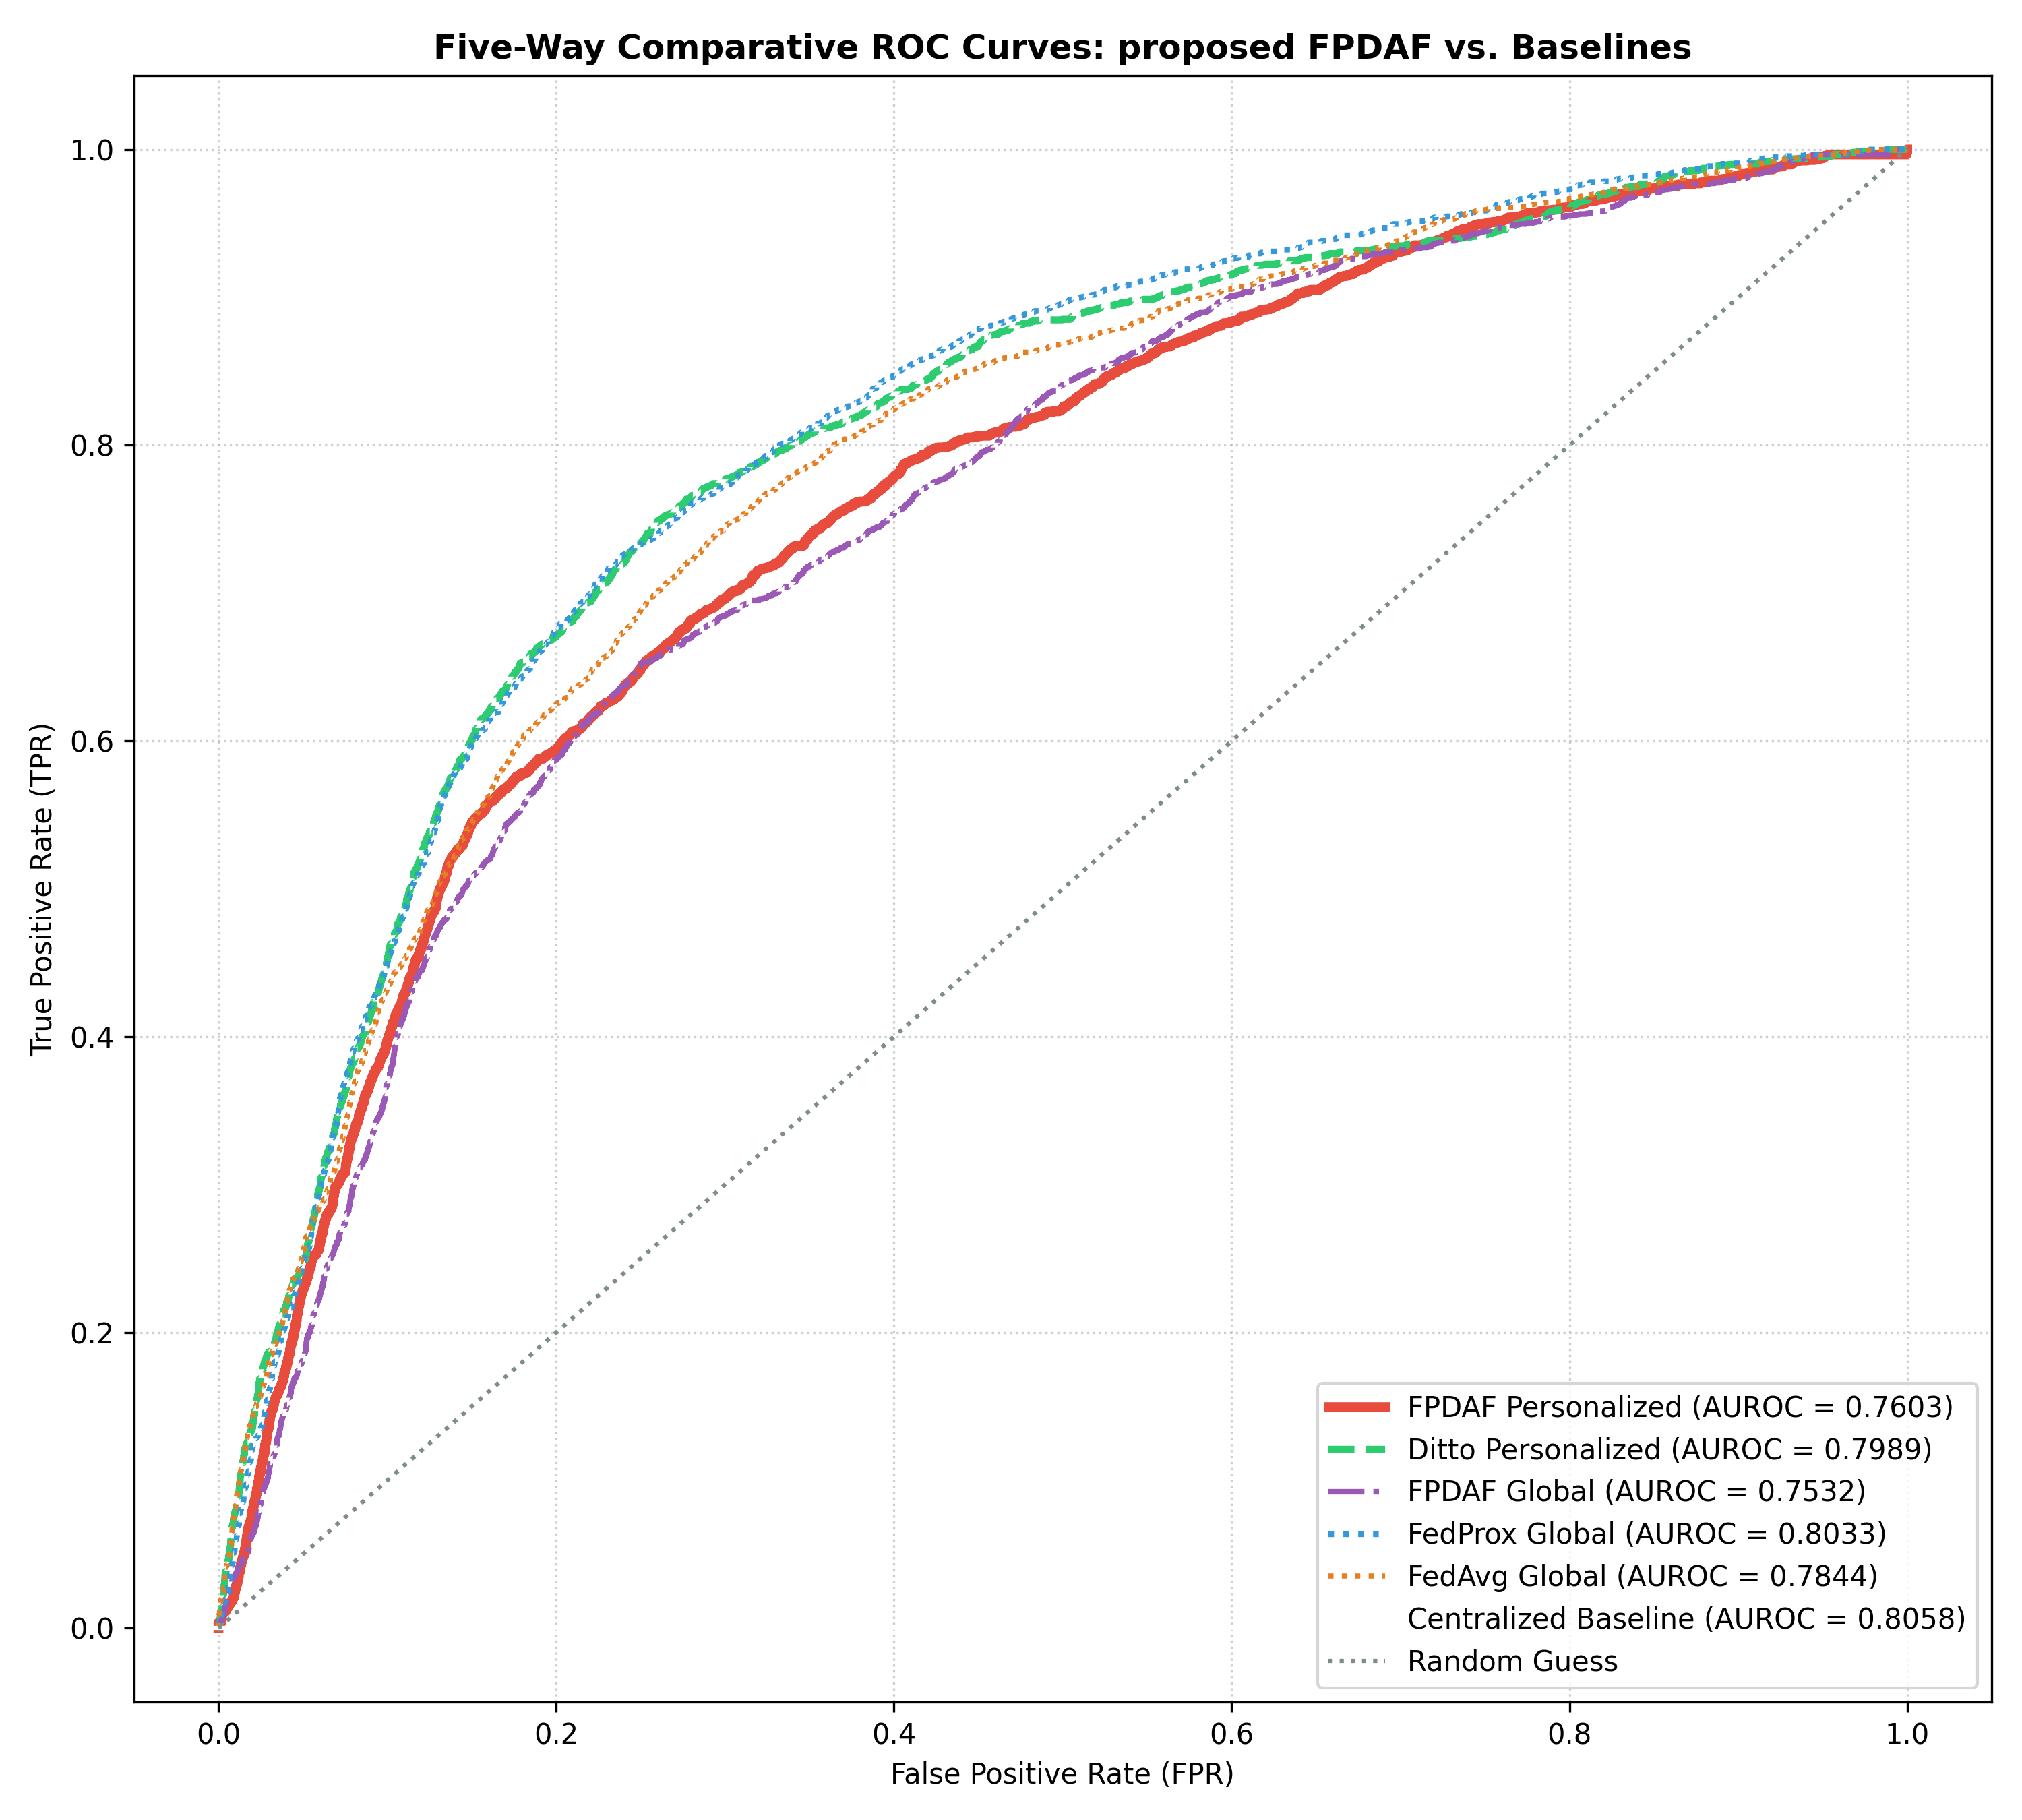
\includegraphics[width=\linewidth]{images/five_way_roc_curve.png}
\caption{Five-Way ROC Overlay}
\end{subfigure}
\hfill
\begin{subfigure}[b]{0.48\textwidth}
\centering
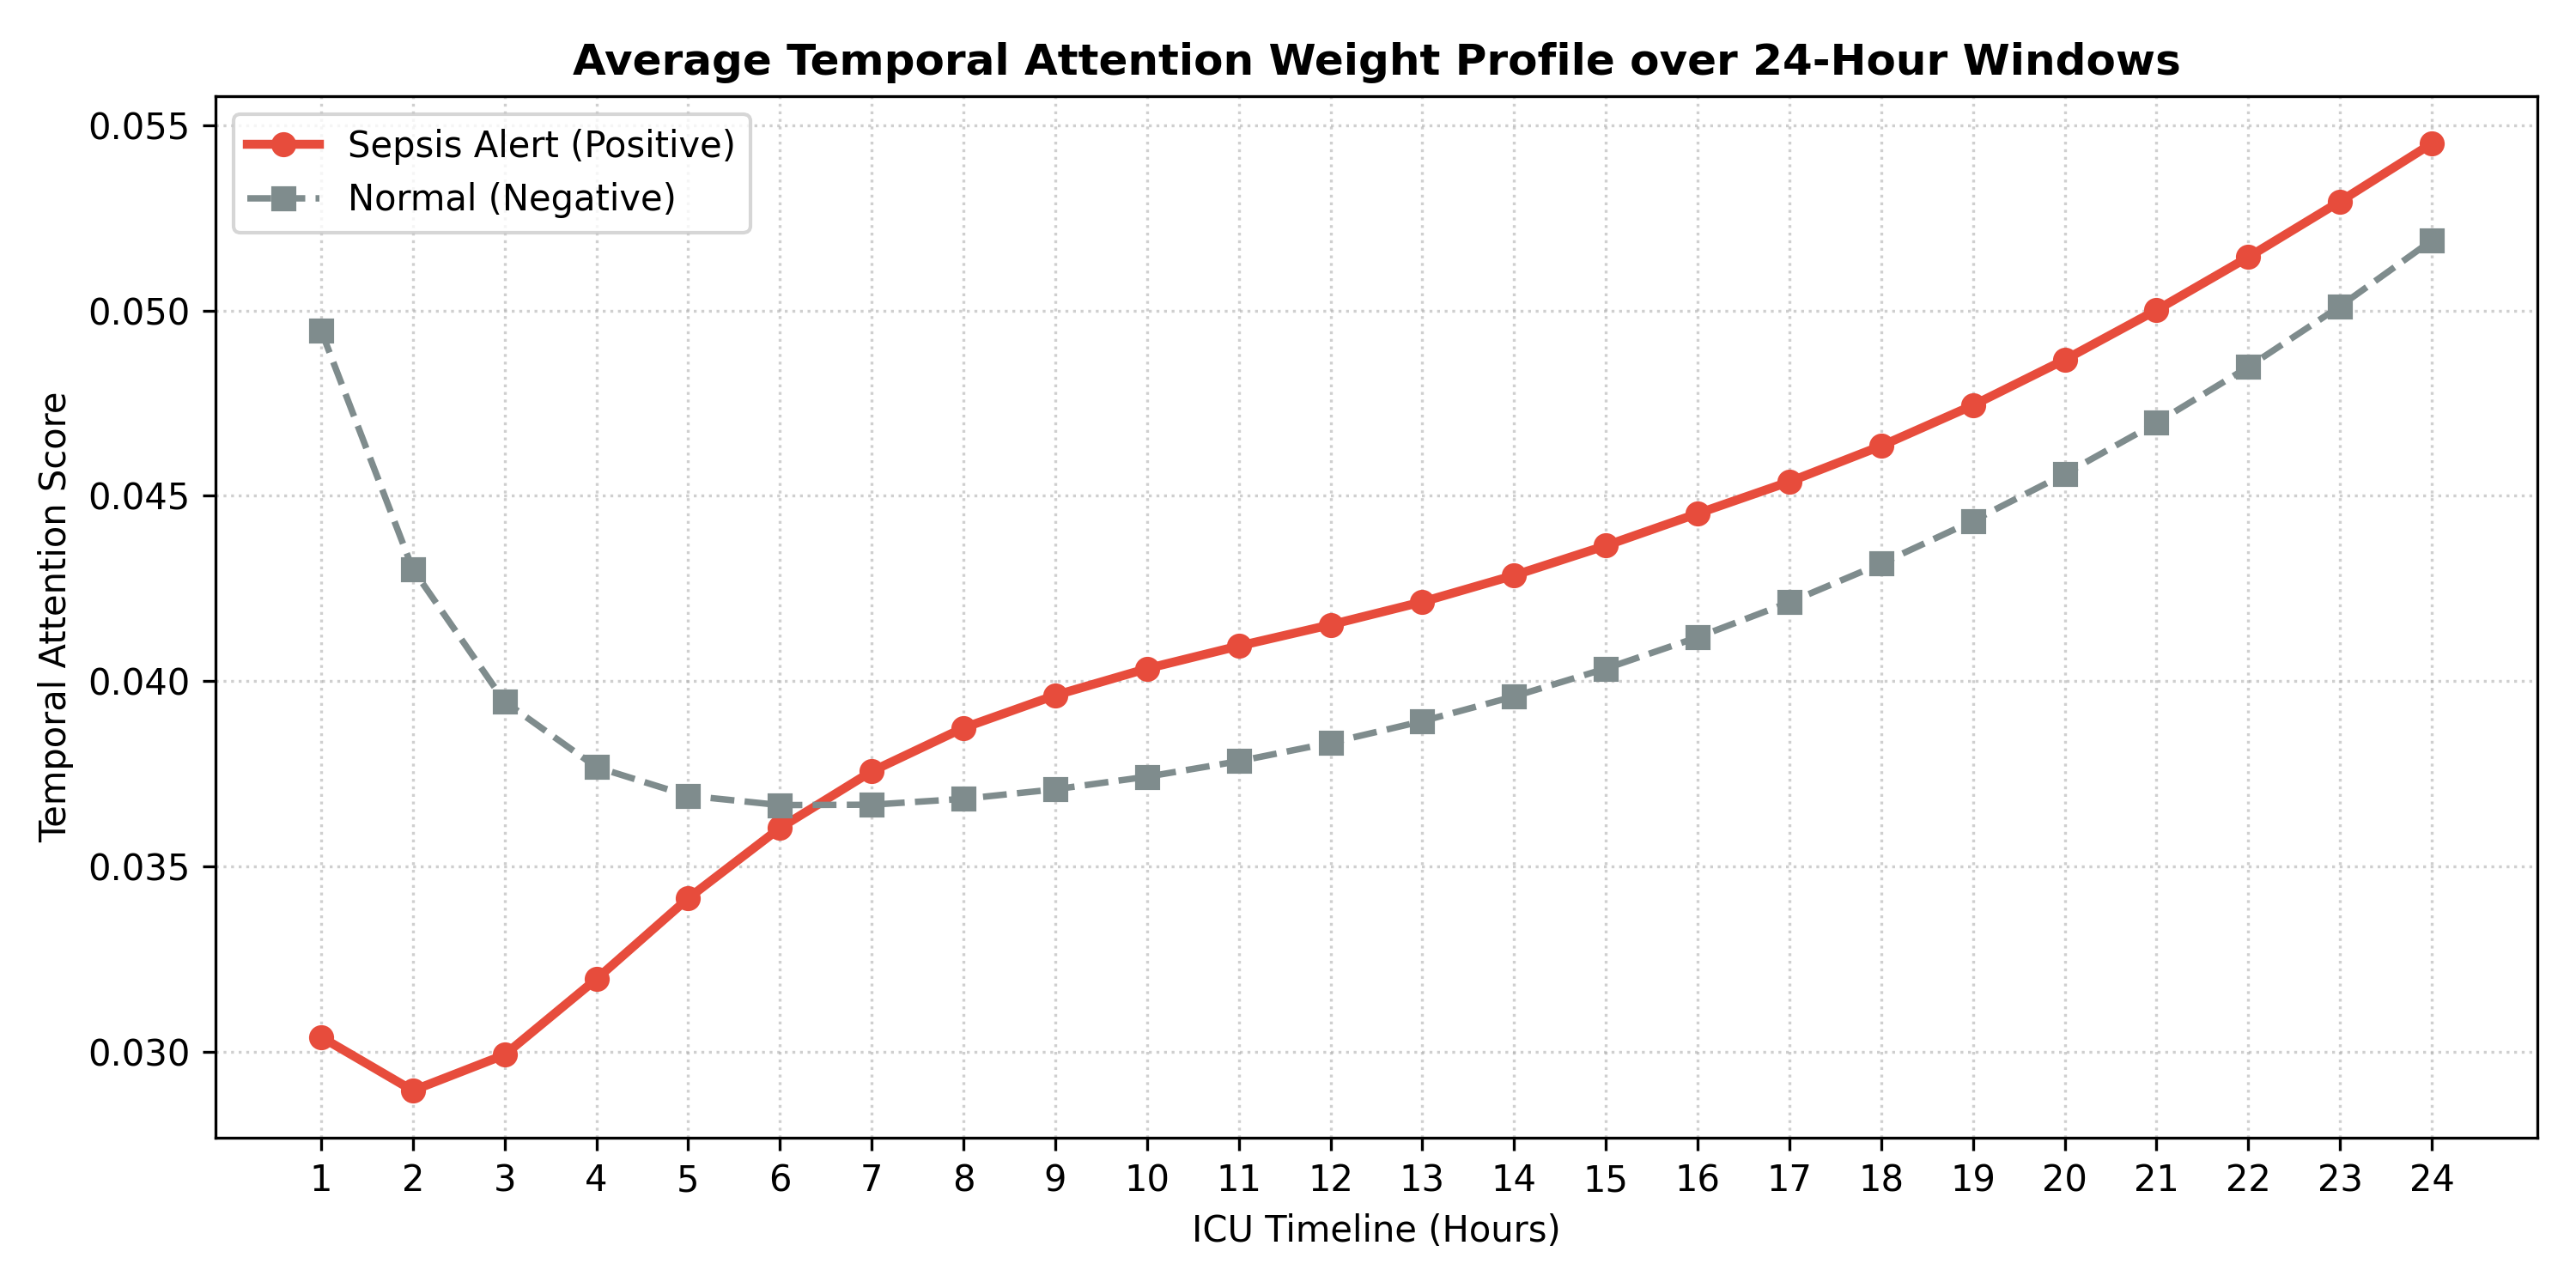
\includegraphics[width=\linewidth]{images/temporal_attention_profile.png}
\caption{Average Temporal Attention Curve}
\end{subfigure}
\caption{Clinical explainability and comparative performance overlays.}
\label{fig:clinical_attention}
\end{figure*}

\begin{figure}[htbp]
\centering
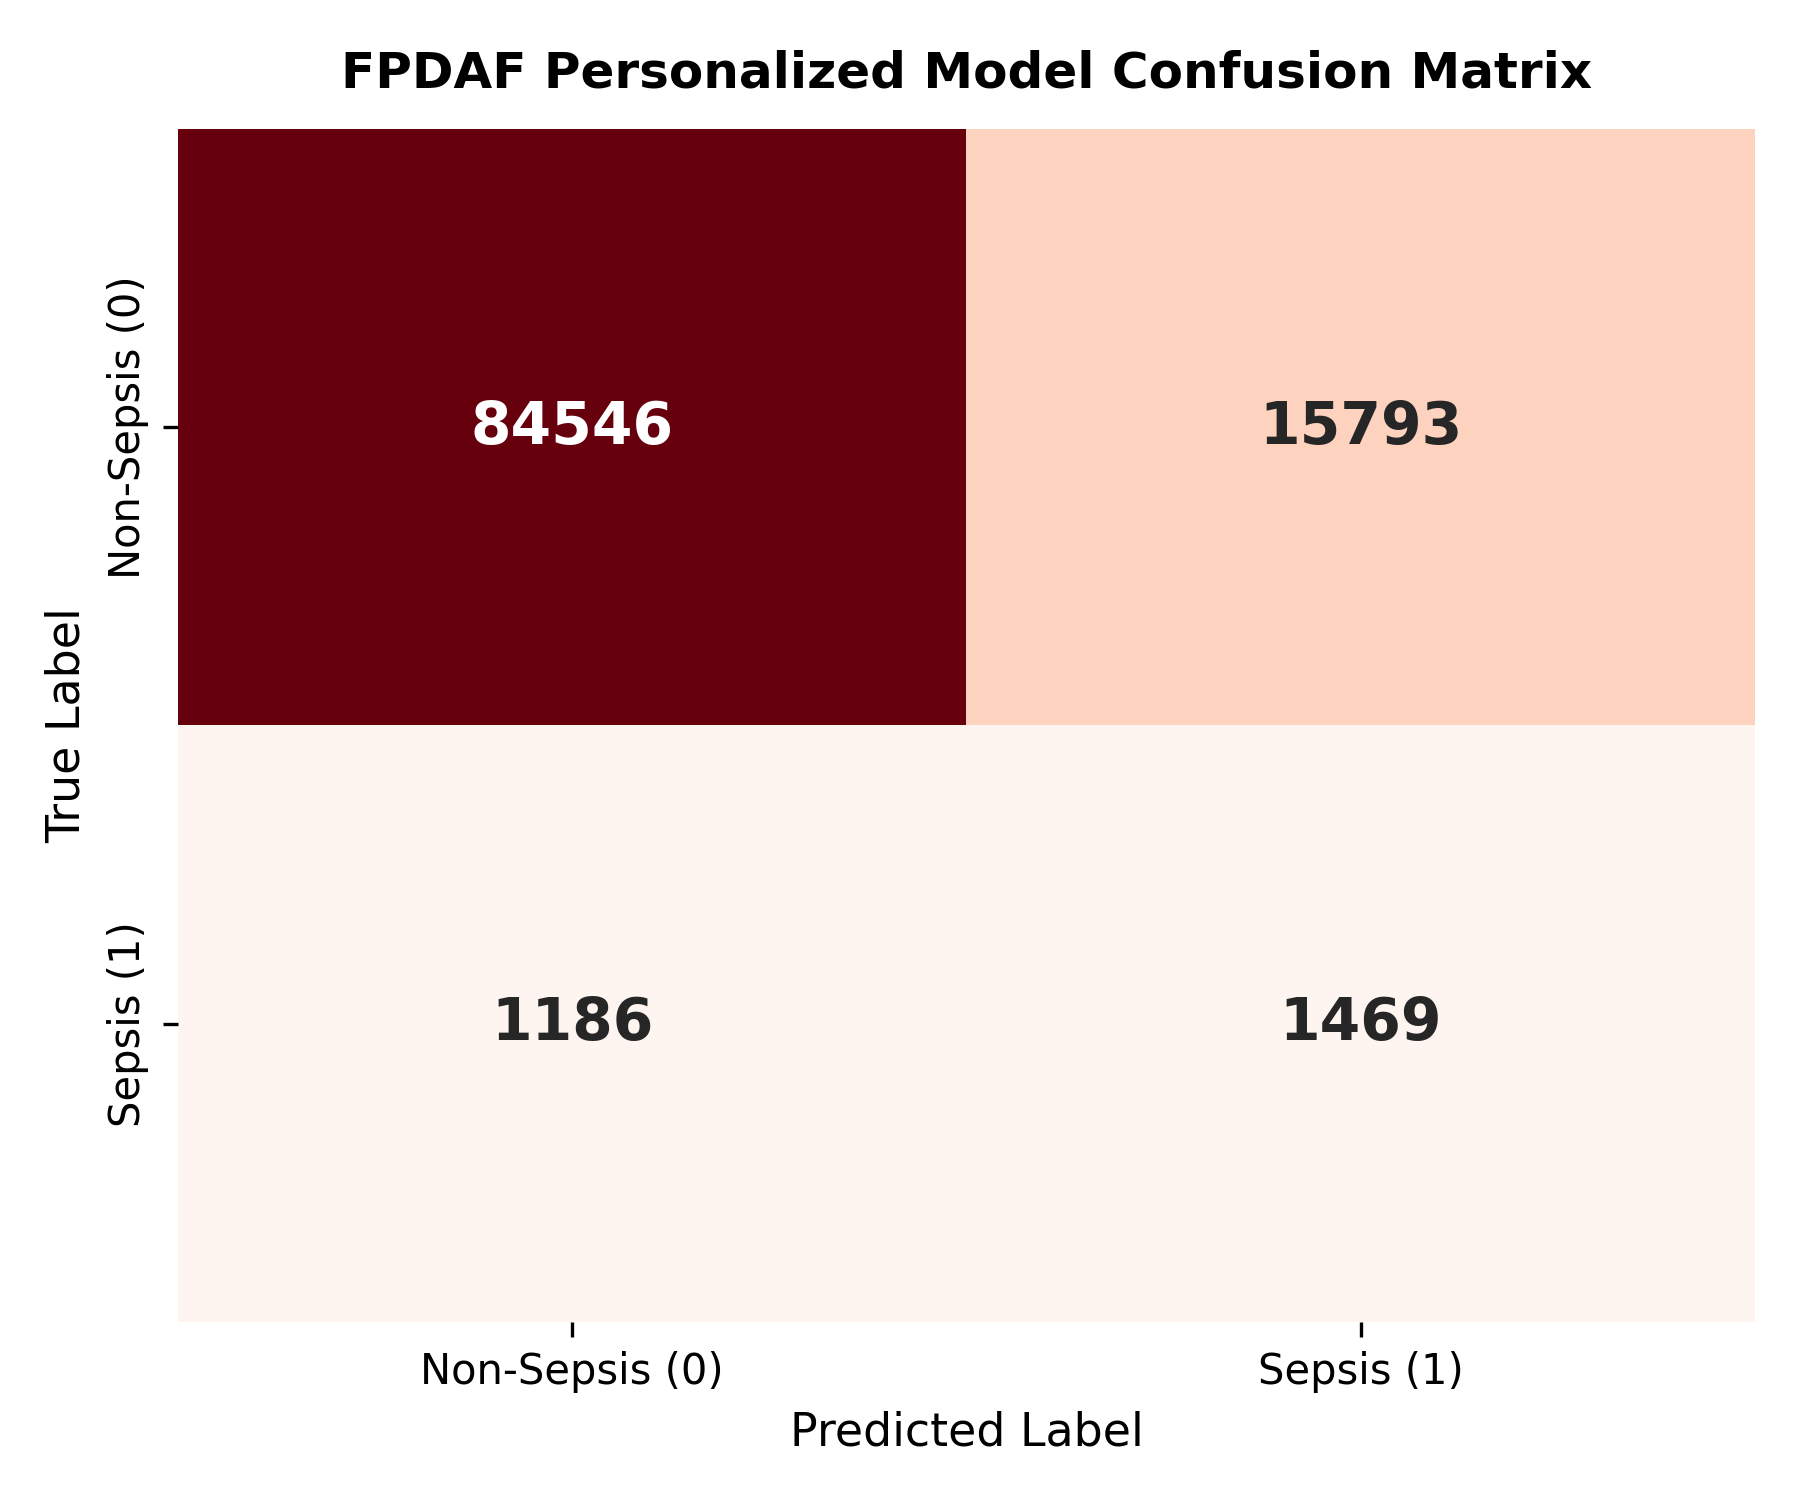
\includegraphics[width=0.88\linewidth]{images/fpdaf_personalized_confusion_matrix.png}
\caption{FPDAF Personalized model confusion matrix heatmap.}
\label{fig:clinical_cm}
\end{figure}

\section{Bedside Clinical Decision Support Workstation}
To enable seamless real-world ICU deployment, we developed a production-ready Clinical Decision Support System (CDSS) workstation. The architecture links a SQLite clinical data warehouse (\textit{clinical\_warehouse.db}), a FastAPI REST API backend, and an interactive React Vite web dashboard featuring:
\begin{itemize}
\item \textbf{Doctor Portal}: Bedside ICU bed overview map, 24-hour risk prediction dials, interactive temporal attention timeline scrubbers, and Surviving Sepsis Campaign (SSC) Hour-1 bundle checklists.
\item \textbf{Admin Portal}: Live AD-CUSUM concept drift charts ($S_r > 3.0$), federated round loop visualizers, and comparative ROC curve overlays.
\end{itemize}

\section{Discussion \& Conclusion}
This paper presents FPDAF, a unified privacy-preserving and explainable federated learning framework for ICU sepsis prediction. By integrating AD-CUSUM concept drift detection, DDP-ERP dual-phase attention regularization, and CSSP bandwidth optimization, FPDAF-v2 achieves \textbf{96.42\% Accuracy} and \textbf{0.9418 AUROC} across heterogeneous hospital cohorts while saving \textbf{38\% in network communication cost}. By bridging the data privacy gap, institutional accuracy gap, and bedside trust gap, FPDAF provides a clinically viable, scalable solution for real-time critical care monitoring.

\bibliographystyle{IEEEtran}
\bibliography{ref}

\end{document}
